%!TEX root = SISC_elastic_3d.tex
\subsection{Gaussian source}\label{gaussian_source}
In this section, we present the numerical experiments to illustrate that there is no obvious artifacts are generated by the curvilinear interface. Specifically, we test the problem in the computational domain
\begin{equation*}
\left\{
\begin{aligned}
& x^{c,(1)} = 2000 r^{(1)}\\
& x^{c,(2)} = 2000 r^{(2)}\\
& x^{c,(3)} = r^{(3)} \theta_i\big(r^{(1)}, r^{(2)}\big) + (1-r^{(3)}) \theta_b\big(r^{(1)},r^{(2)}\big)
\end{aligned}
\right.
\end{equation*}
for coarse domain $\Omega^c$. Here, $0\leq r^{(1)}, r^{(2)}, r^{(3)}\leq 1$, $\theta_i$ is the interface surface geometry,
\begin{equation}\label{interface_gausian}
\theta_i\big(r^{(1)},r^{(2)}\big) = 800+20\sin(4\pi r^{(1)})+20\cos(4\pi r^{(2)}),
\end{equation}
and 
$\theta_b$ is the bottom surface geometry,
\begin{equation*}
\theta_b\big(r^{(1)},r^{(2)}\big) = 0.
\end{equation*}
As for the fine domain $\Omega^f$, it chooses to be
\begin{equation*}
\left\{
\begin{aligned}
& x^{f,(1)} = 2000 r^{(1)}\\
& x^{f,(2)} = 2000 r^{(2)}\\
& x^{f,(3)} = r^{(3)}\theta_t\big(r^{(1)},r^{(2)}\big) + (1-r^{(3)})\theta_i\big(r^{(1)},r^{(2)}\big),
\end{aligned}
\right.
\end{equation*}
where $0\leq r^{(1)}, r^{(2)}, r^{(3)}\leq 1$, $\theta_t$ is the top surface geometry,
\begin{equation*}
\theta_t\big(r^{(1)},r^{(2)}\big) = 1000,
\end{equation*}
and $\theta_i$ is the interface geometry which is given in (\ref{interface_gausian}). For both fine and coarse domains, let the density vary according to
\begin{equation*}
\rho(x^{(1)},x^{(2)},x^{(3)}) = 1.5\times 10^3,
\end{equation*}
and material parameters $\mu, \lambda$ satisfy
\begin{equation*}
\mu(x^{(1)},x^{(2)},x^{(3)}) = 1.5\times 10^9,\ \ 
\lambda(x^{(1)},x^{(2)},x^{(3)})  = 3\times 10^9,
\end{equation*}
respectively. In addition, we impose a Gaussian source on the top surface
\[{\bf g} = (g_1,g_2,g_3)^T ,\]
where, $g_1 = g_2 = 0$, and 
\[g_3 = 10^9 \text{exp}\left(-\left(\frac{t-4/44.2}{1/44.2}\right)^2\right)\text{exp}\left(-\left(\frac{x^{(1)}-1000}{12.5}\right)^2-\left(\frac{x^{(2)}-1000}{12.5}\right)^2\right).\]

Homogeneous Dirichlet boundary conditions are imposed on other boundaries. The external forcing is chosen to be zero everywhere and the initial conditions are also set to be zero everywhere, ${\bf u} = {\bf 0}$ at $t = 0$.

In the simulation of the reference solution, we choose $n_1 = n_2 = 201, n_3 = 101$. In the experiments for the curvilinear interface with mesh refinement, we have $n_1^{2h} = n_2^{2h} = 101, n_3^{2h} = 41$ and $n_1^h = n_2^h = 201, n_3^h = 21$. The final simulation time is $T = 0.4$.

\begin{figure}[htbp]
	\centering
	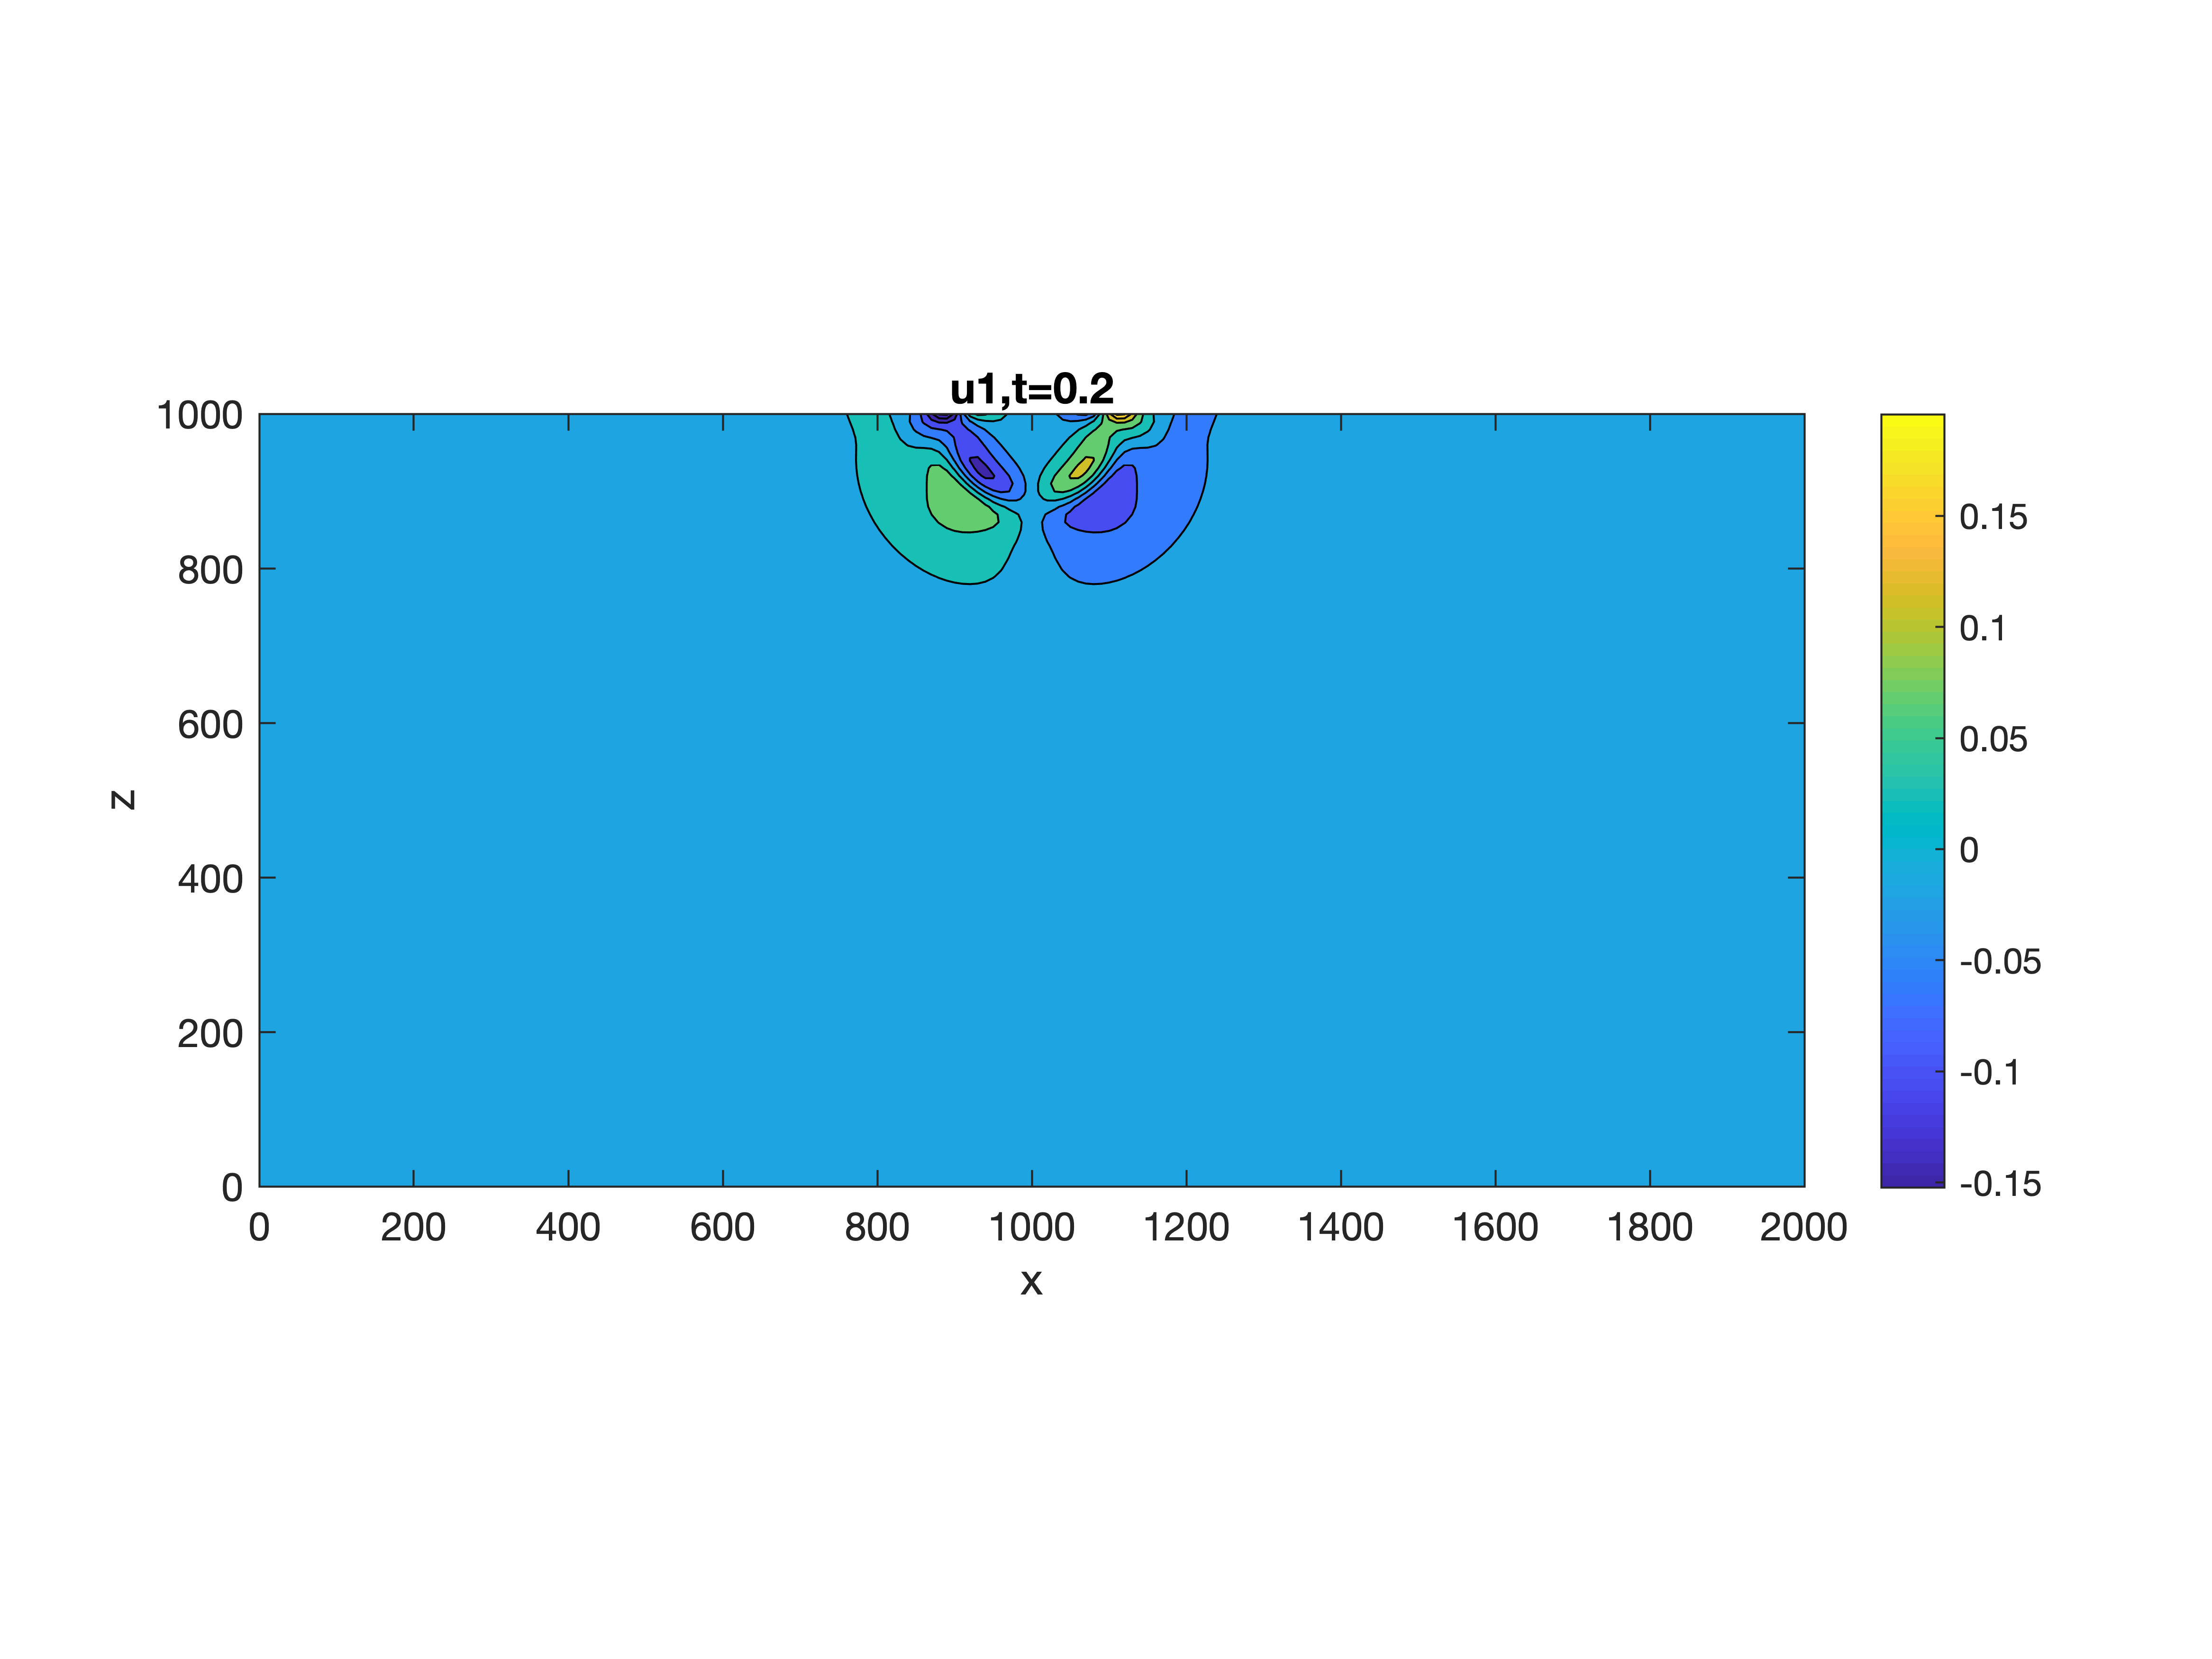
\includegraphics[width=0.4\textwidth,trim={0 2.8cm 0 2.8cm}, clip]{u1_t02_cartesian.png}
	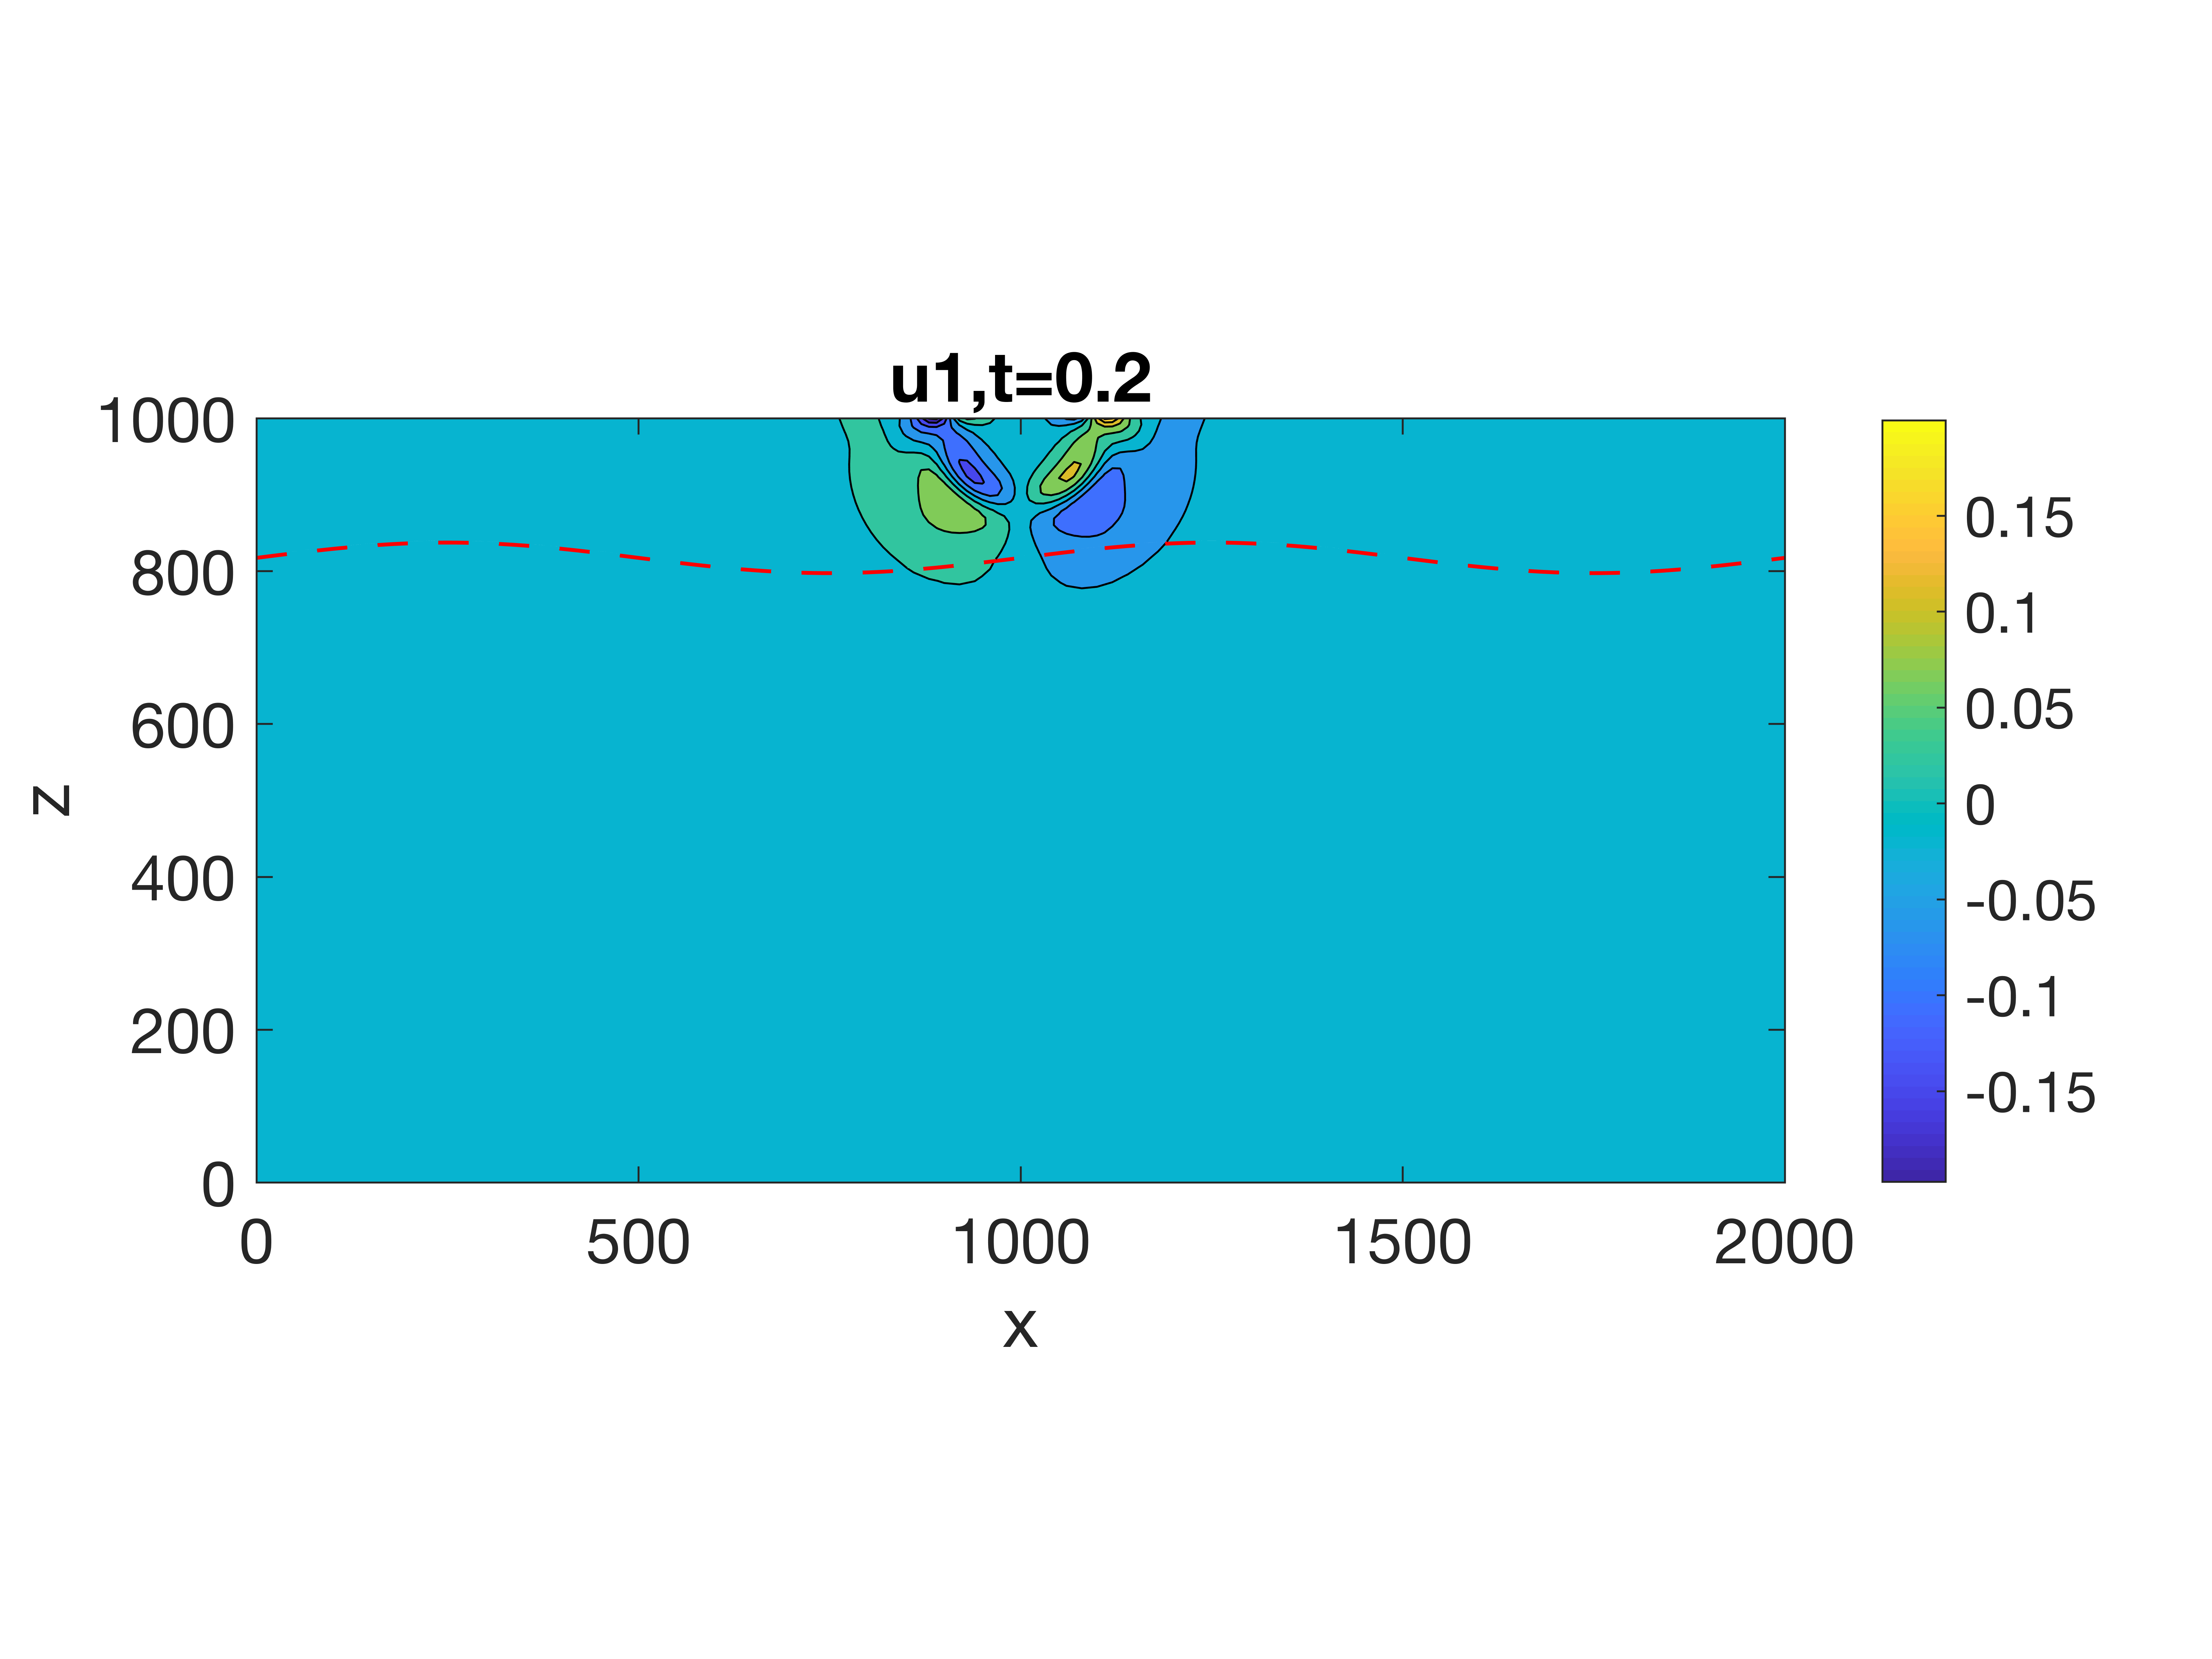
\includegraphics[width=0.4\textwidth,trim={0 2.8cm 0 2.8cm}, clip]{u1_t02_curvi_mr.png}\\
	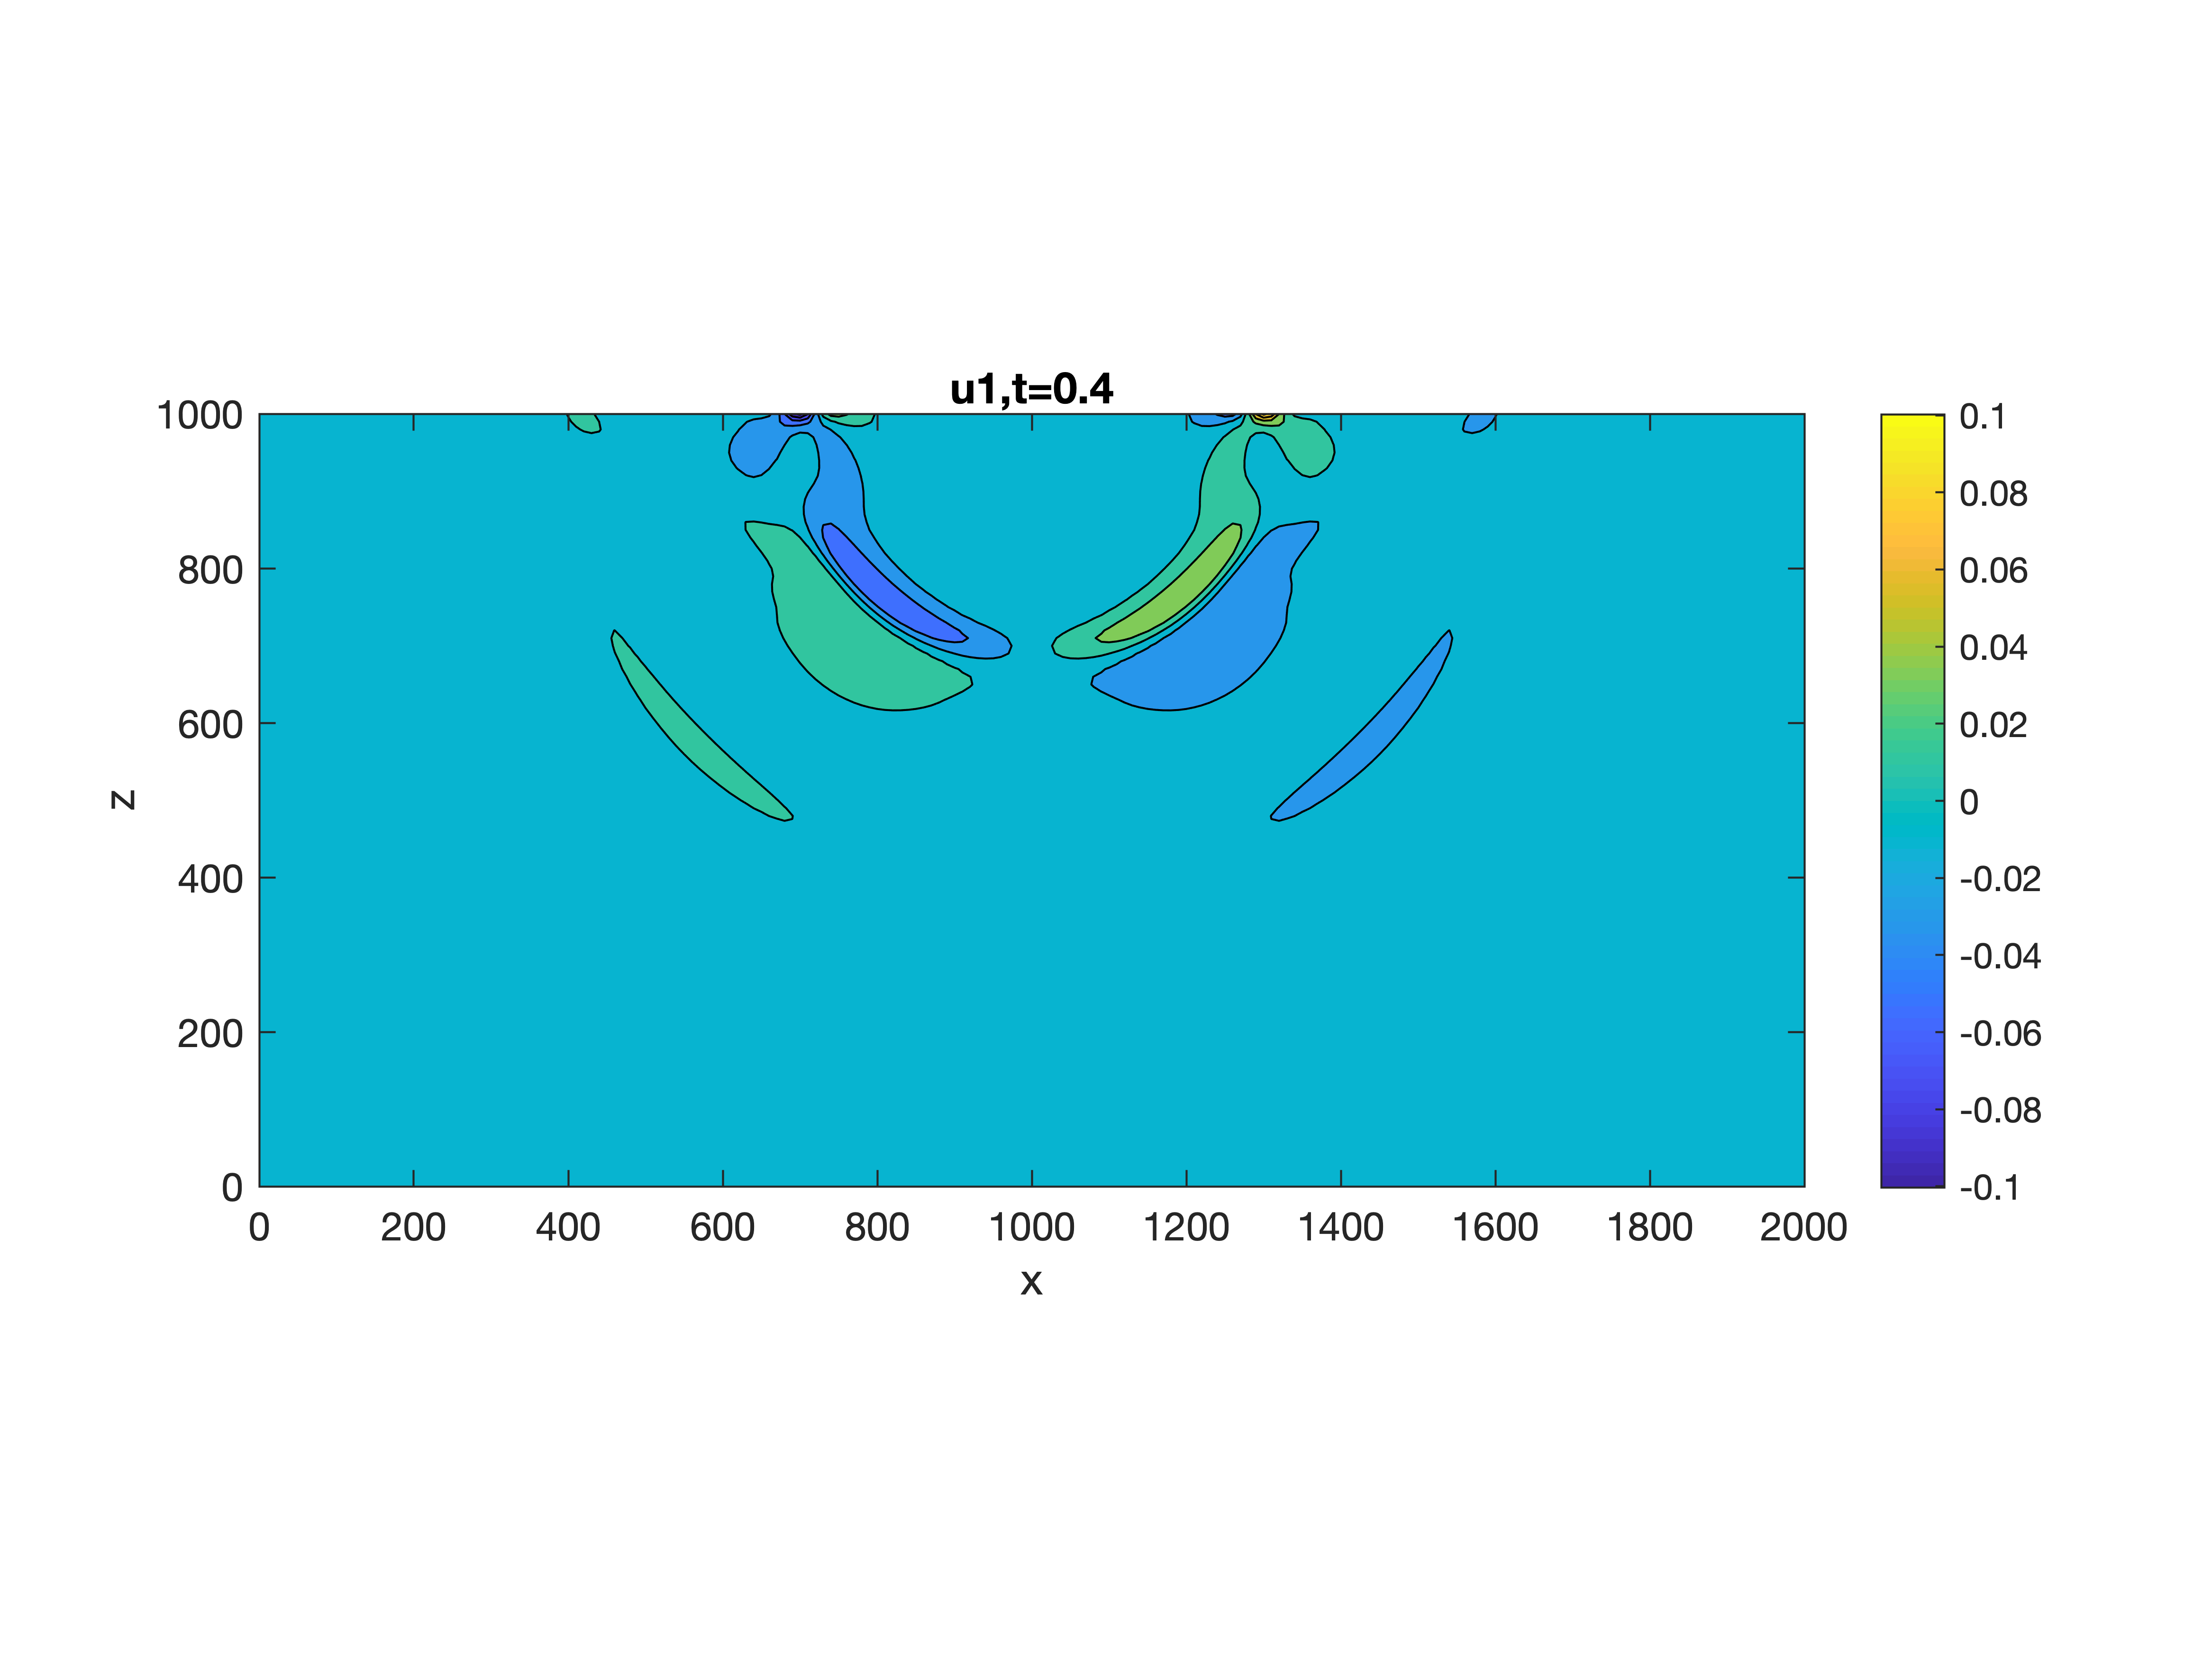
\includegraphics[width=0.4\textwidth,trim={0 2.8cm 0 2.8cm}, clip]{u1_t04_cartesian.png}
	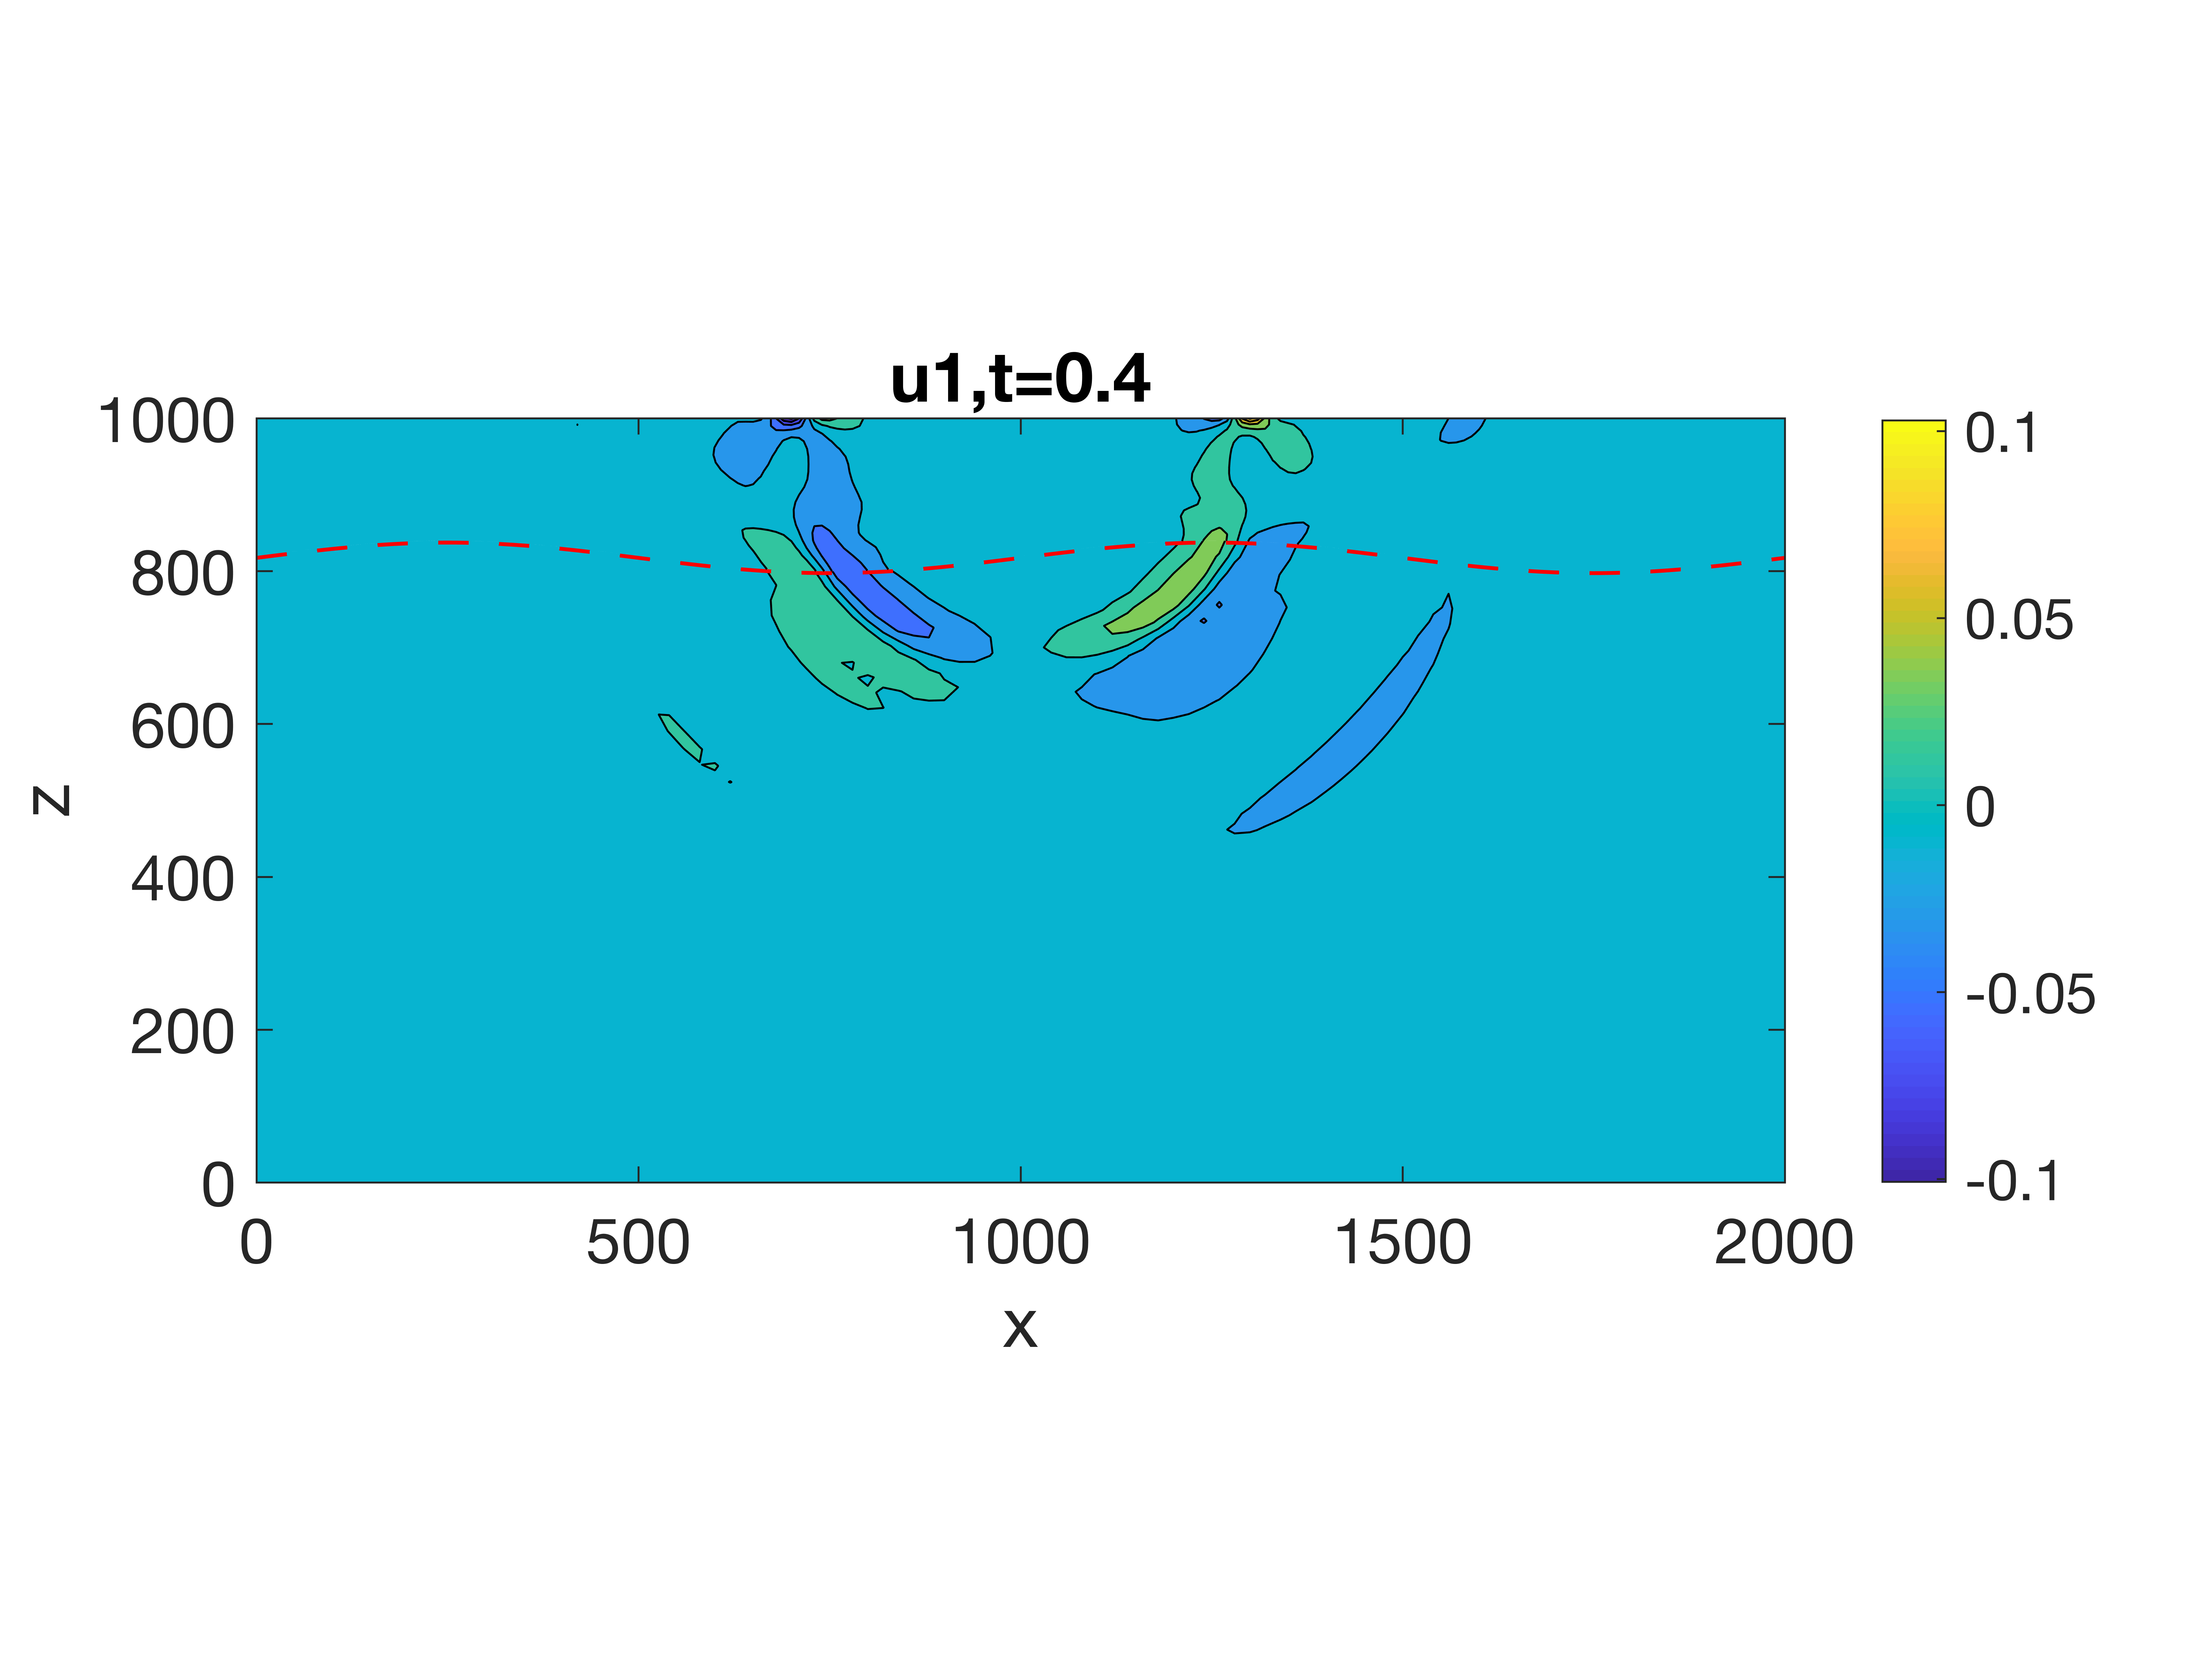
\includegraphics[width=0.4\textwidth,trim={0 2.8cm 0 2.8cm}, clip]{u1_t04_curvi_mr.png}
\caption{The graphs for $u_1$. In the two figures on the left, we show reference solutions at $t=0.2$ and $t=0.4$, computed on a Cartesian mesh without mesh refinement interface. On the right, the two figures show the solutions computed on a curvilinear mesh with a curved mesh refinement interface at $t=0.2$ and $t=0.4$. The curved interfaces are marked with the red dash lines. Note that $x,z$ in the graph correspond to $x^{(1)}, x^{(3)}$ respectively.}
\label{u1}
\end{figure}

%\begin{figure}[htbp]
%	\centering
%	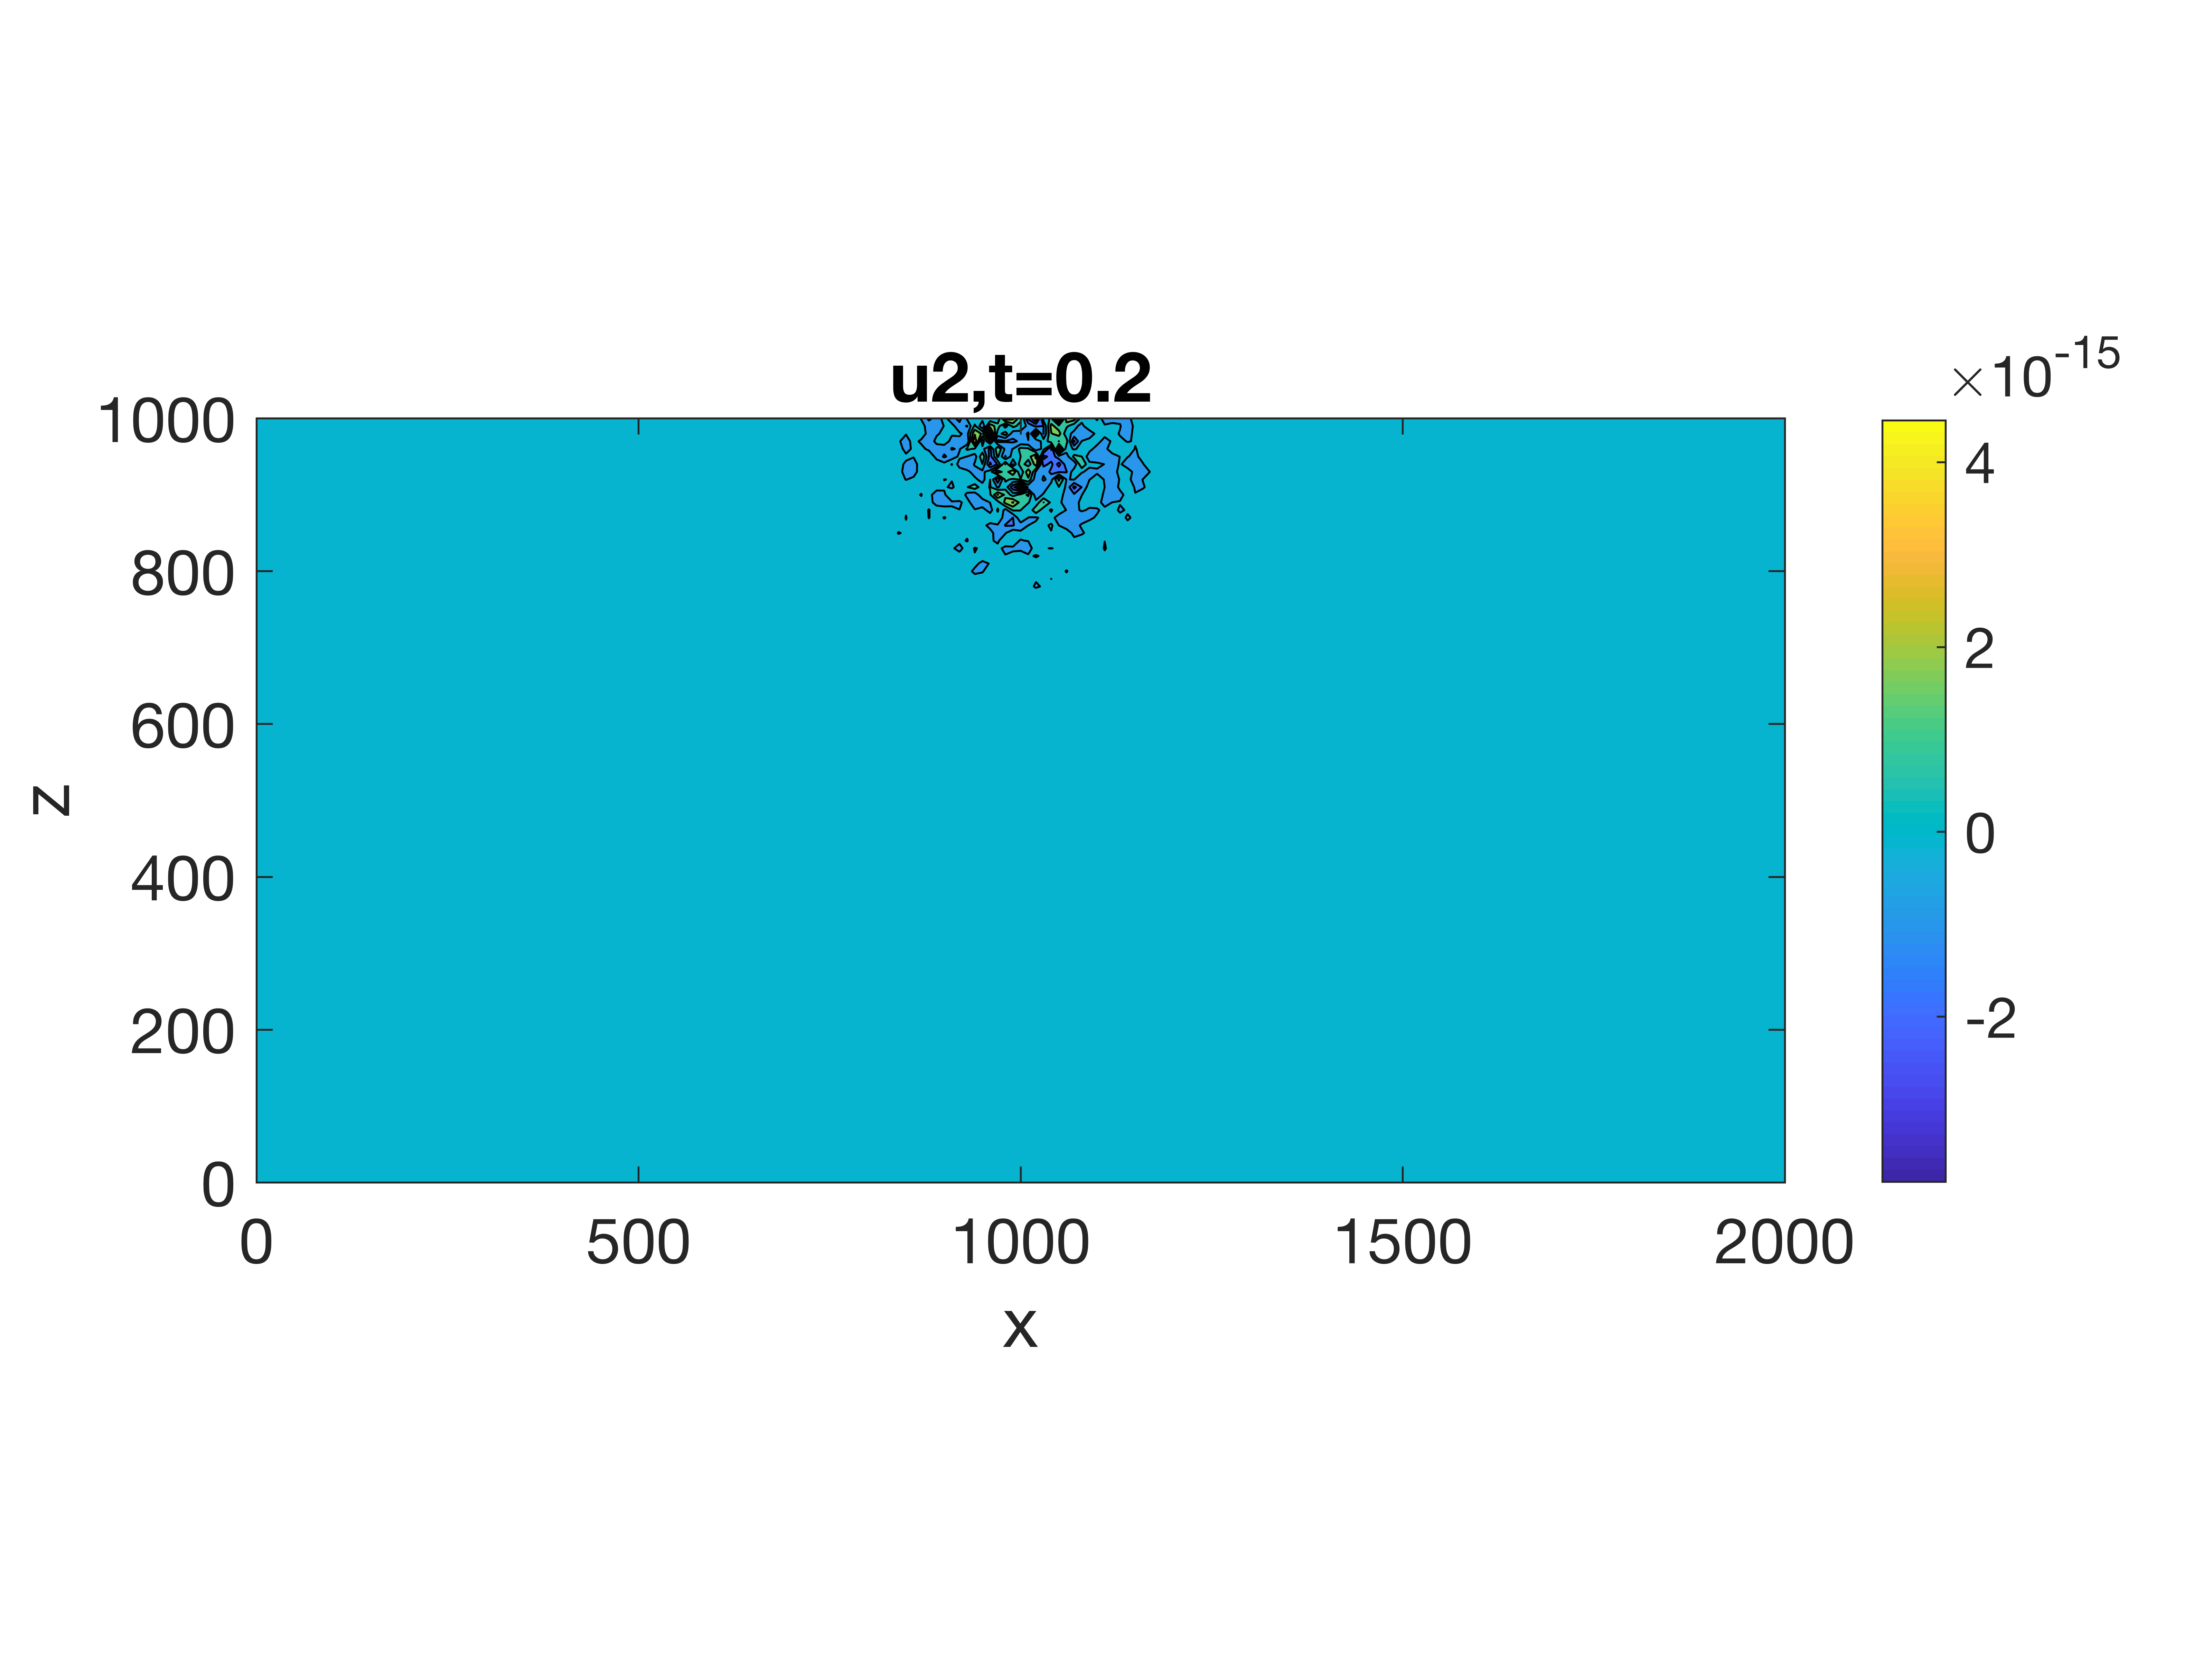
\includegraphics[width=0.4\textwidth,trim={0 2.8cm 0 2.8cm}, clip]{u2_t02_cartesian.png}
%	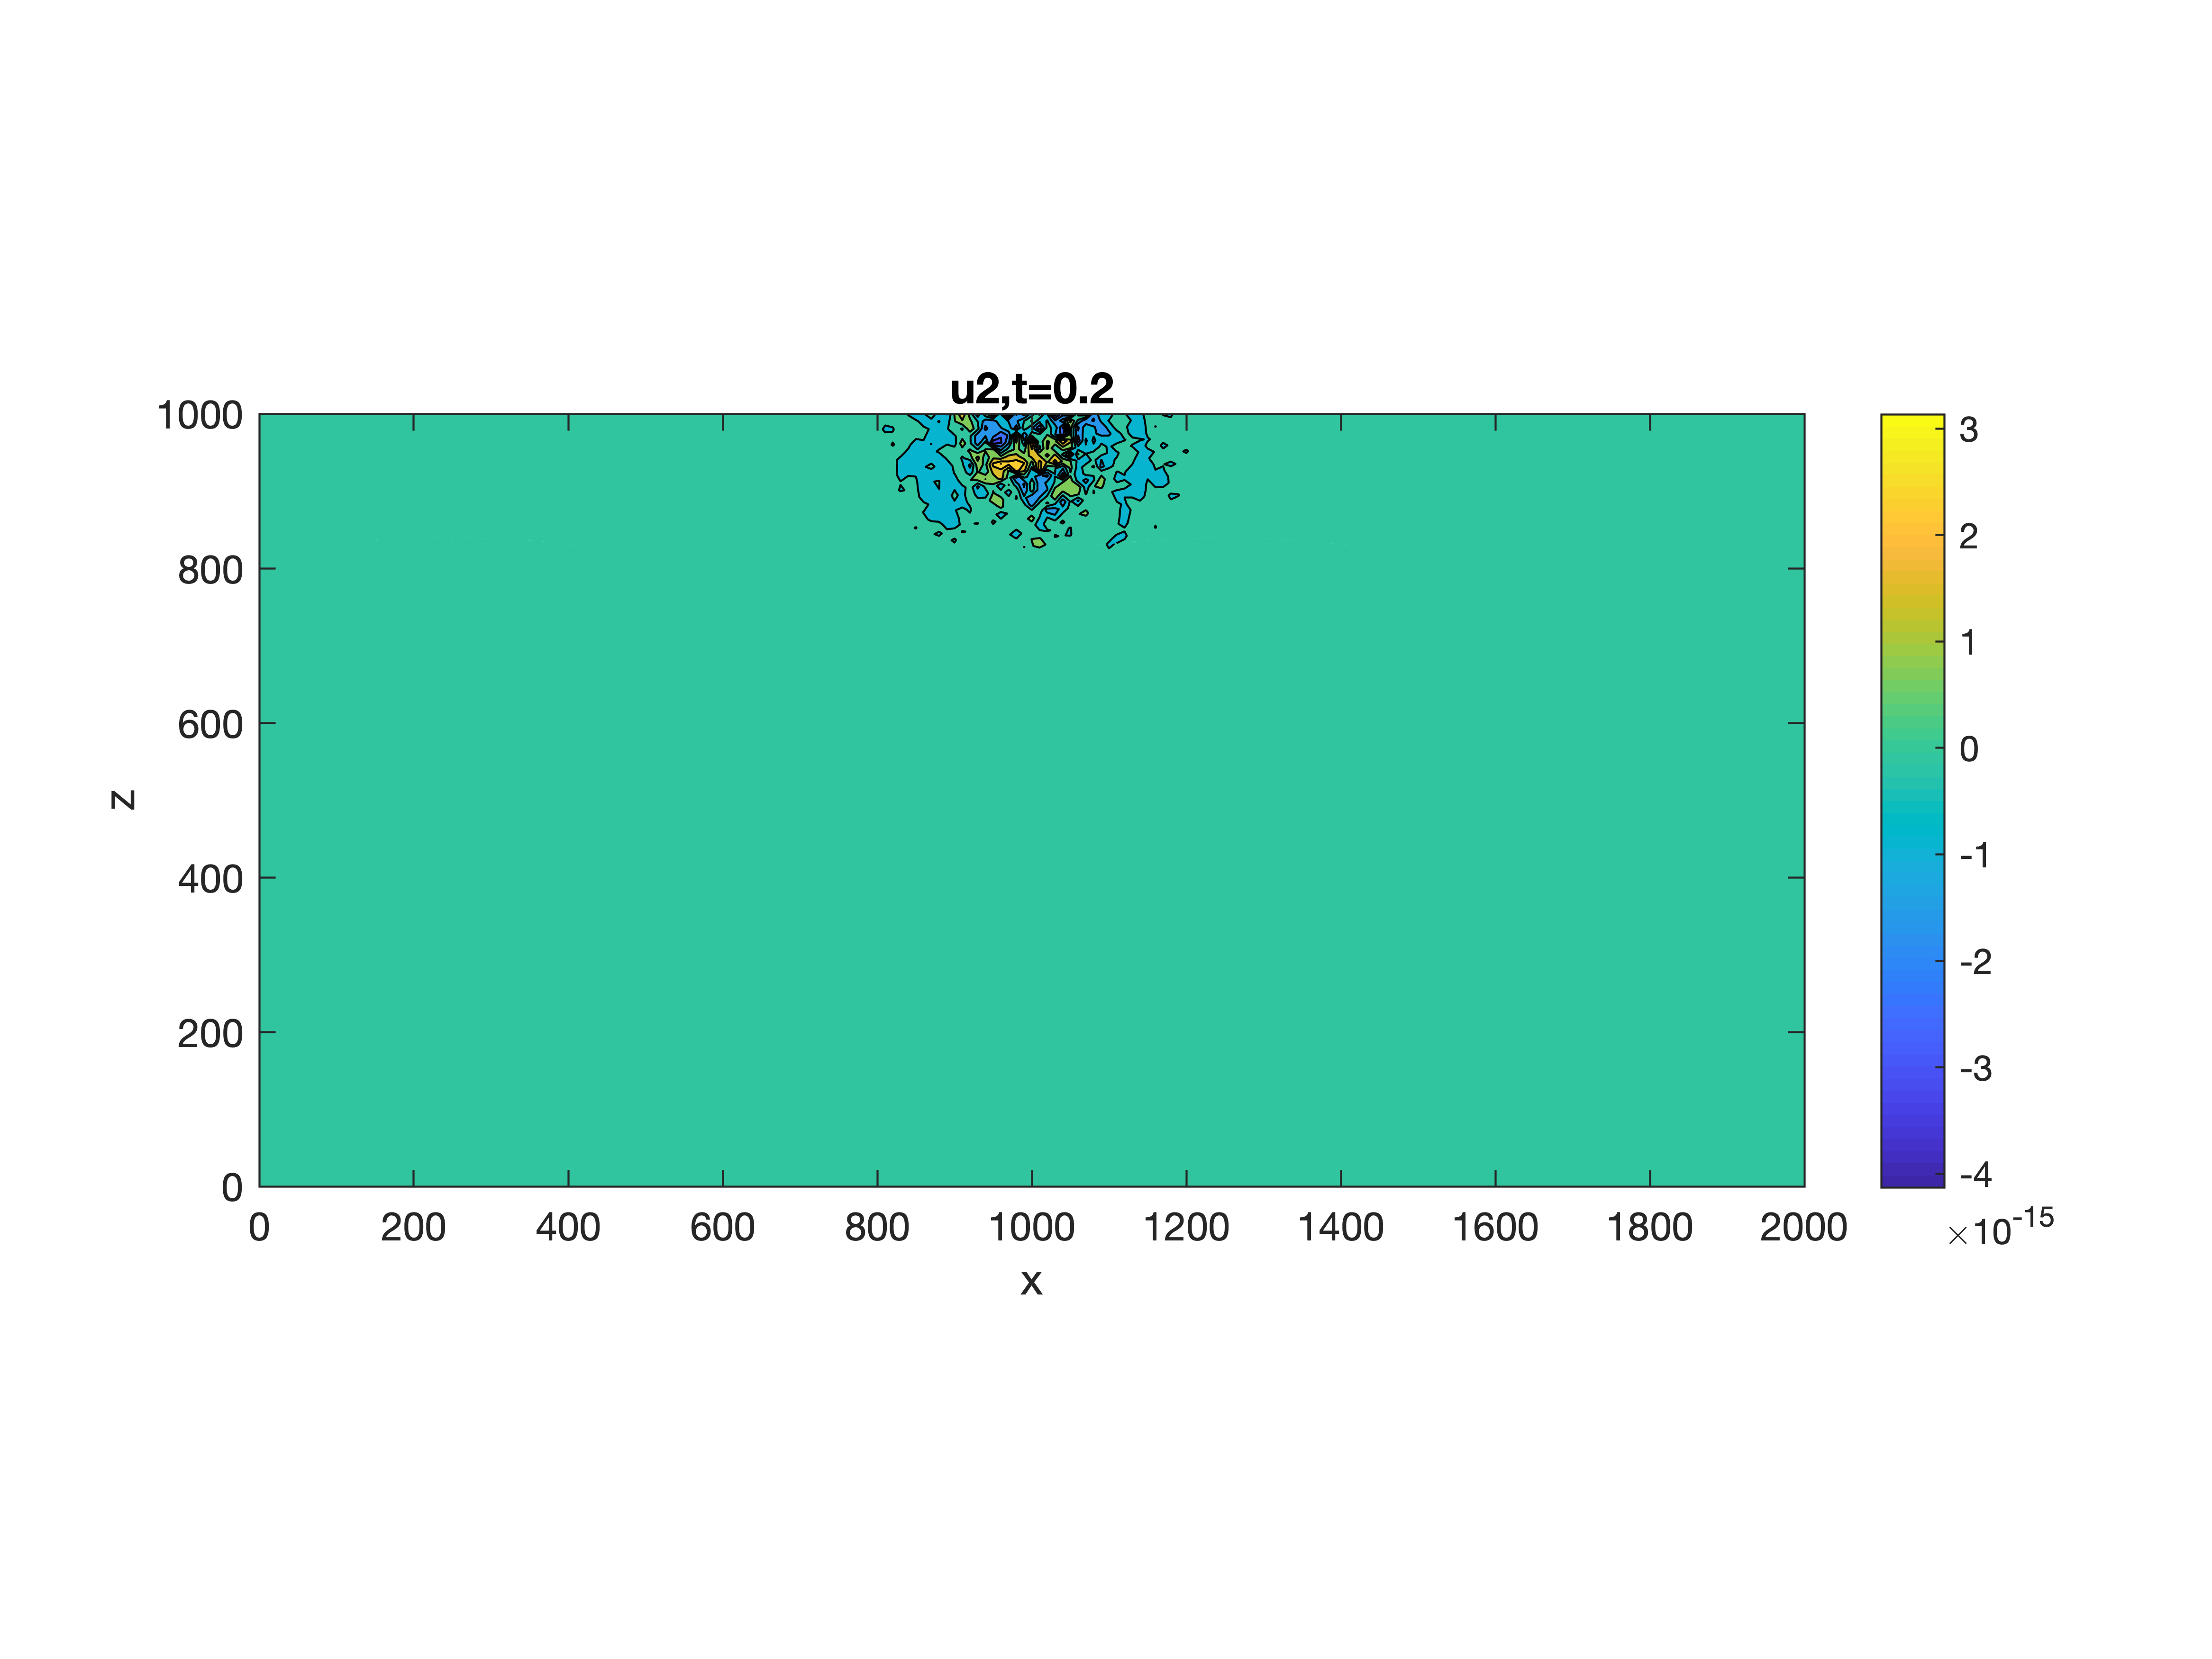
\includegraphics[width=0.4\textwidth,trim={0 2.8cm 0 2.8cm}, clip]{u2_t02_curvi_mr.png}\\
%	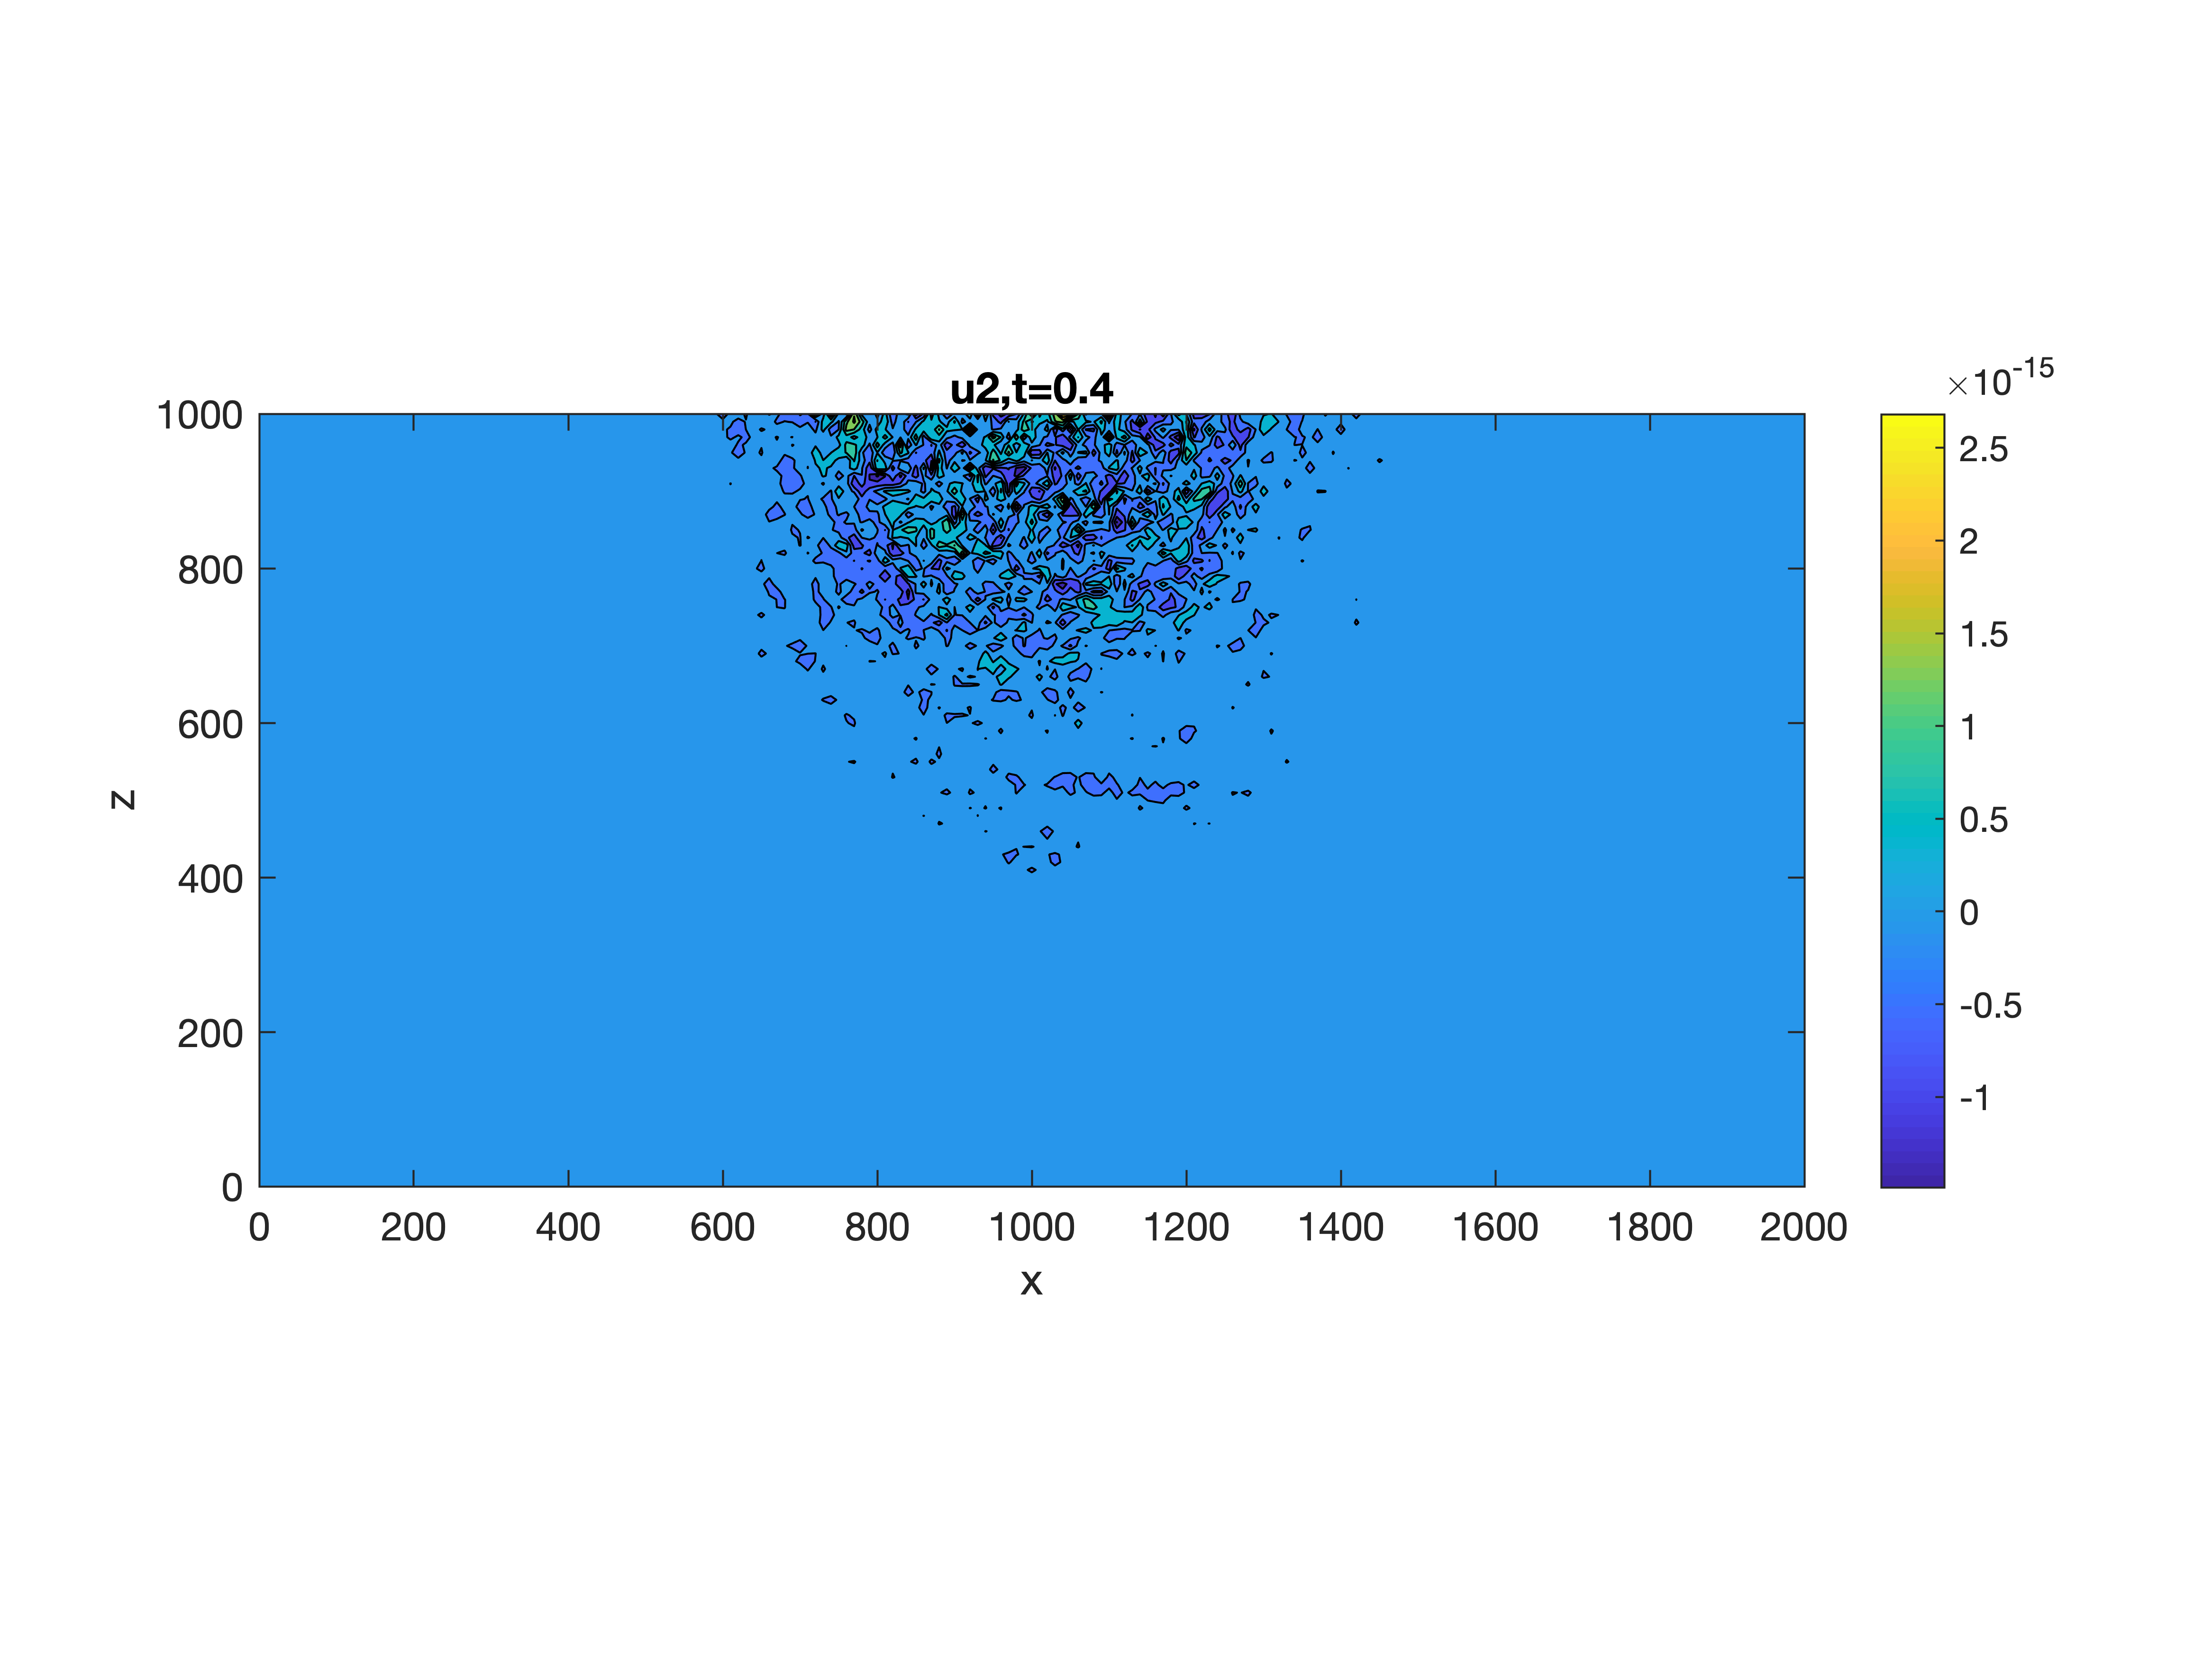
\includegraphics[width=0.4\textwidth,trim={0 2.8cm 0 2.8cm}, clip]{u2_t04_cartesian.png}
%	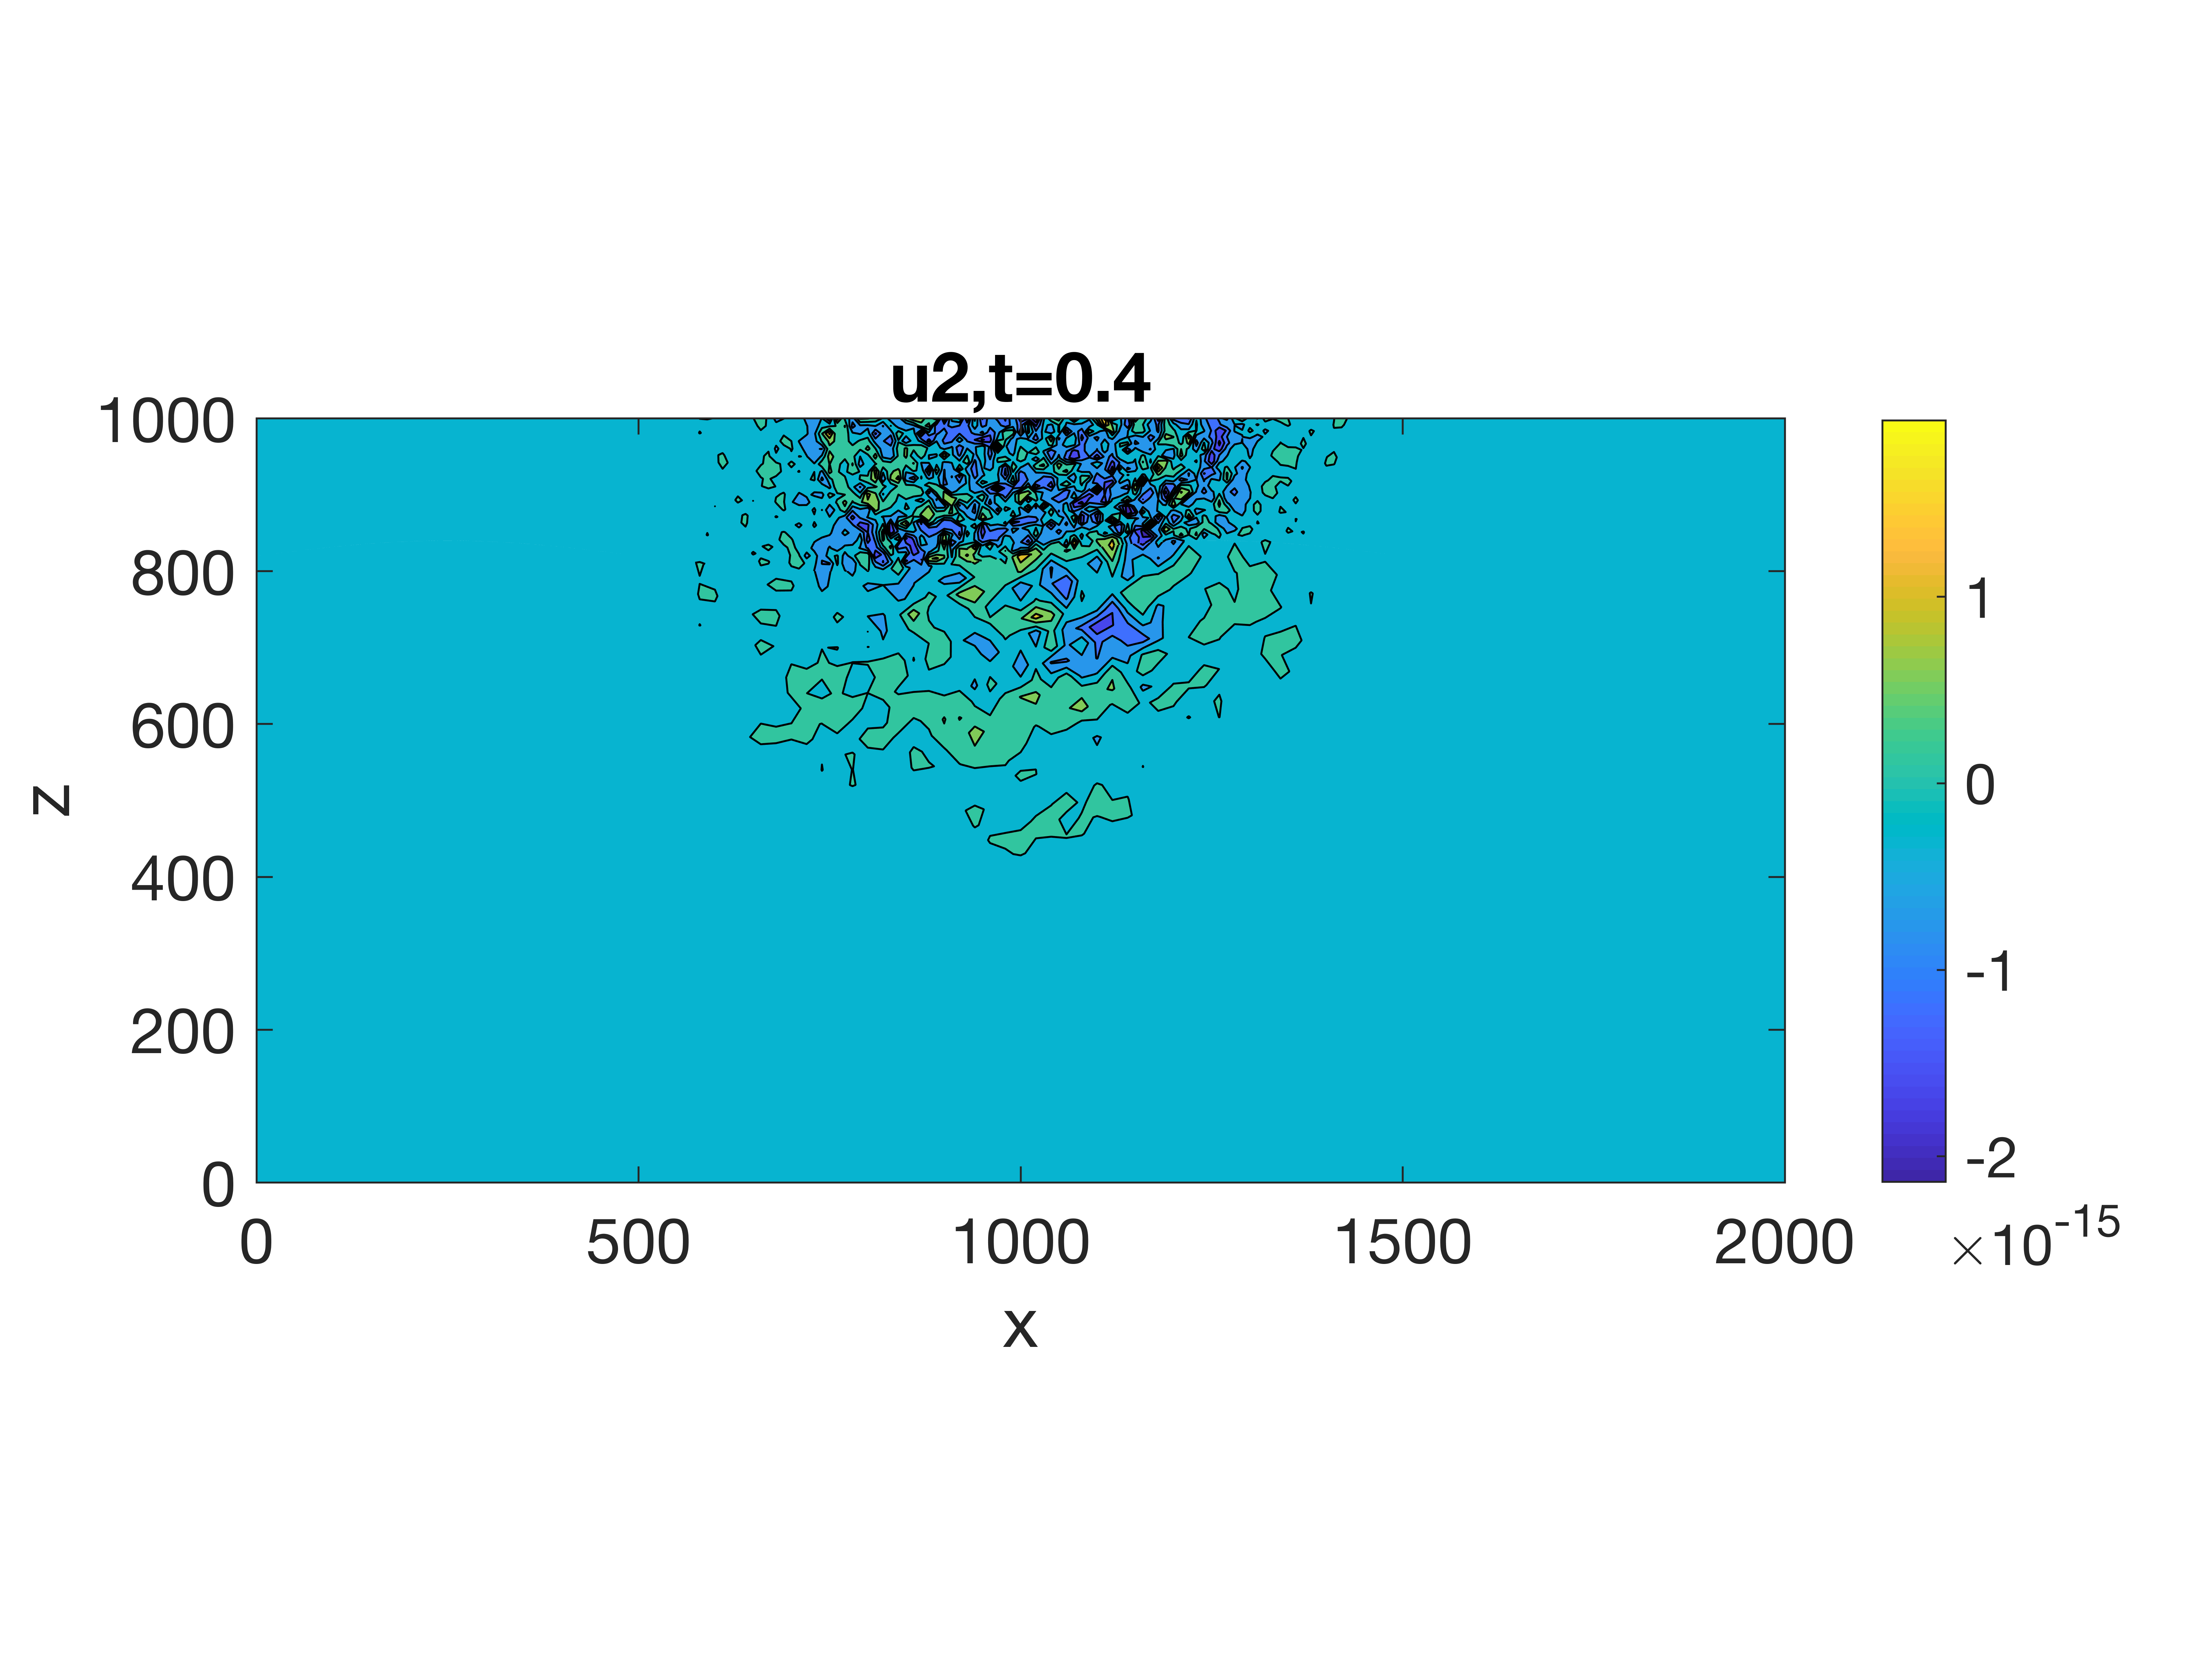
\includegraphics[width=0.4\textwidth,trim={0 2.8cm 0 2.8cm}, clip]{u2_t04_curvi_mr.png}
%	\caption{The graph for $u_2$. From left to right are for Cartesian mesh without mesh refinement interface and curvilinear mesh with mesh refinement interface respectively. From top to bottom are for $t = 0.2$ and $t = 0.4$ respectively. Note that $x,z$ in the graph correspond to $x^{(1)}, x^{(3)}$ respectively.}\label{u2}
%\end{figure}

\begin{figure}[htbp]
	\centering
	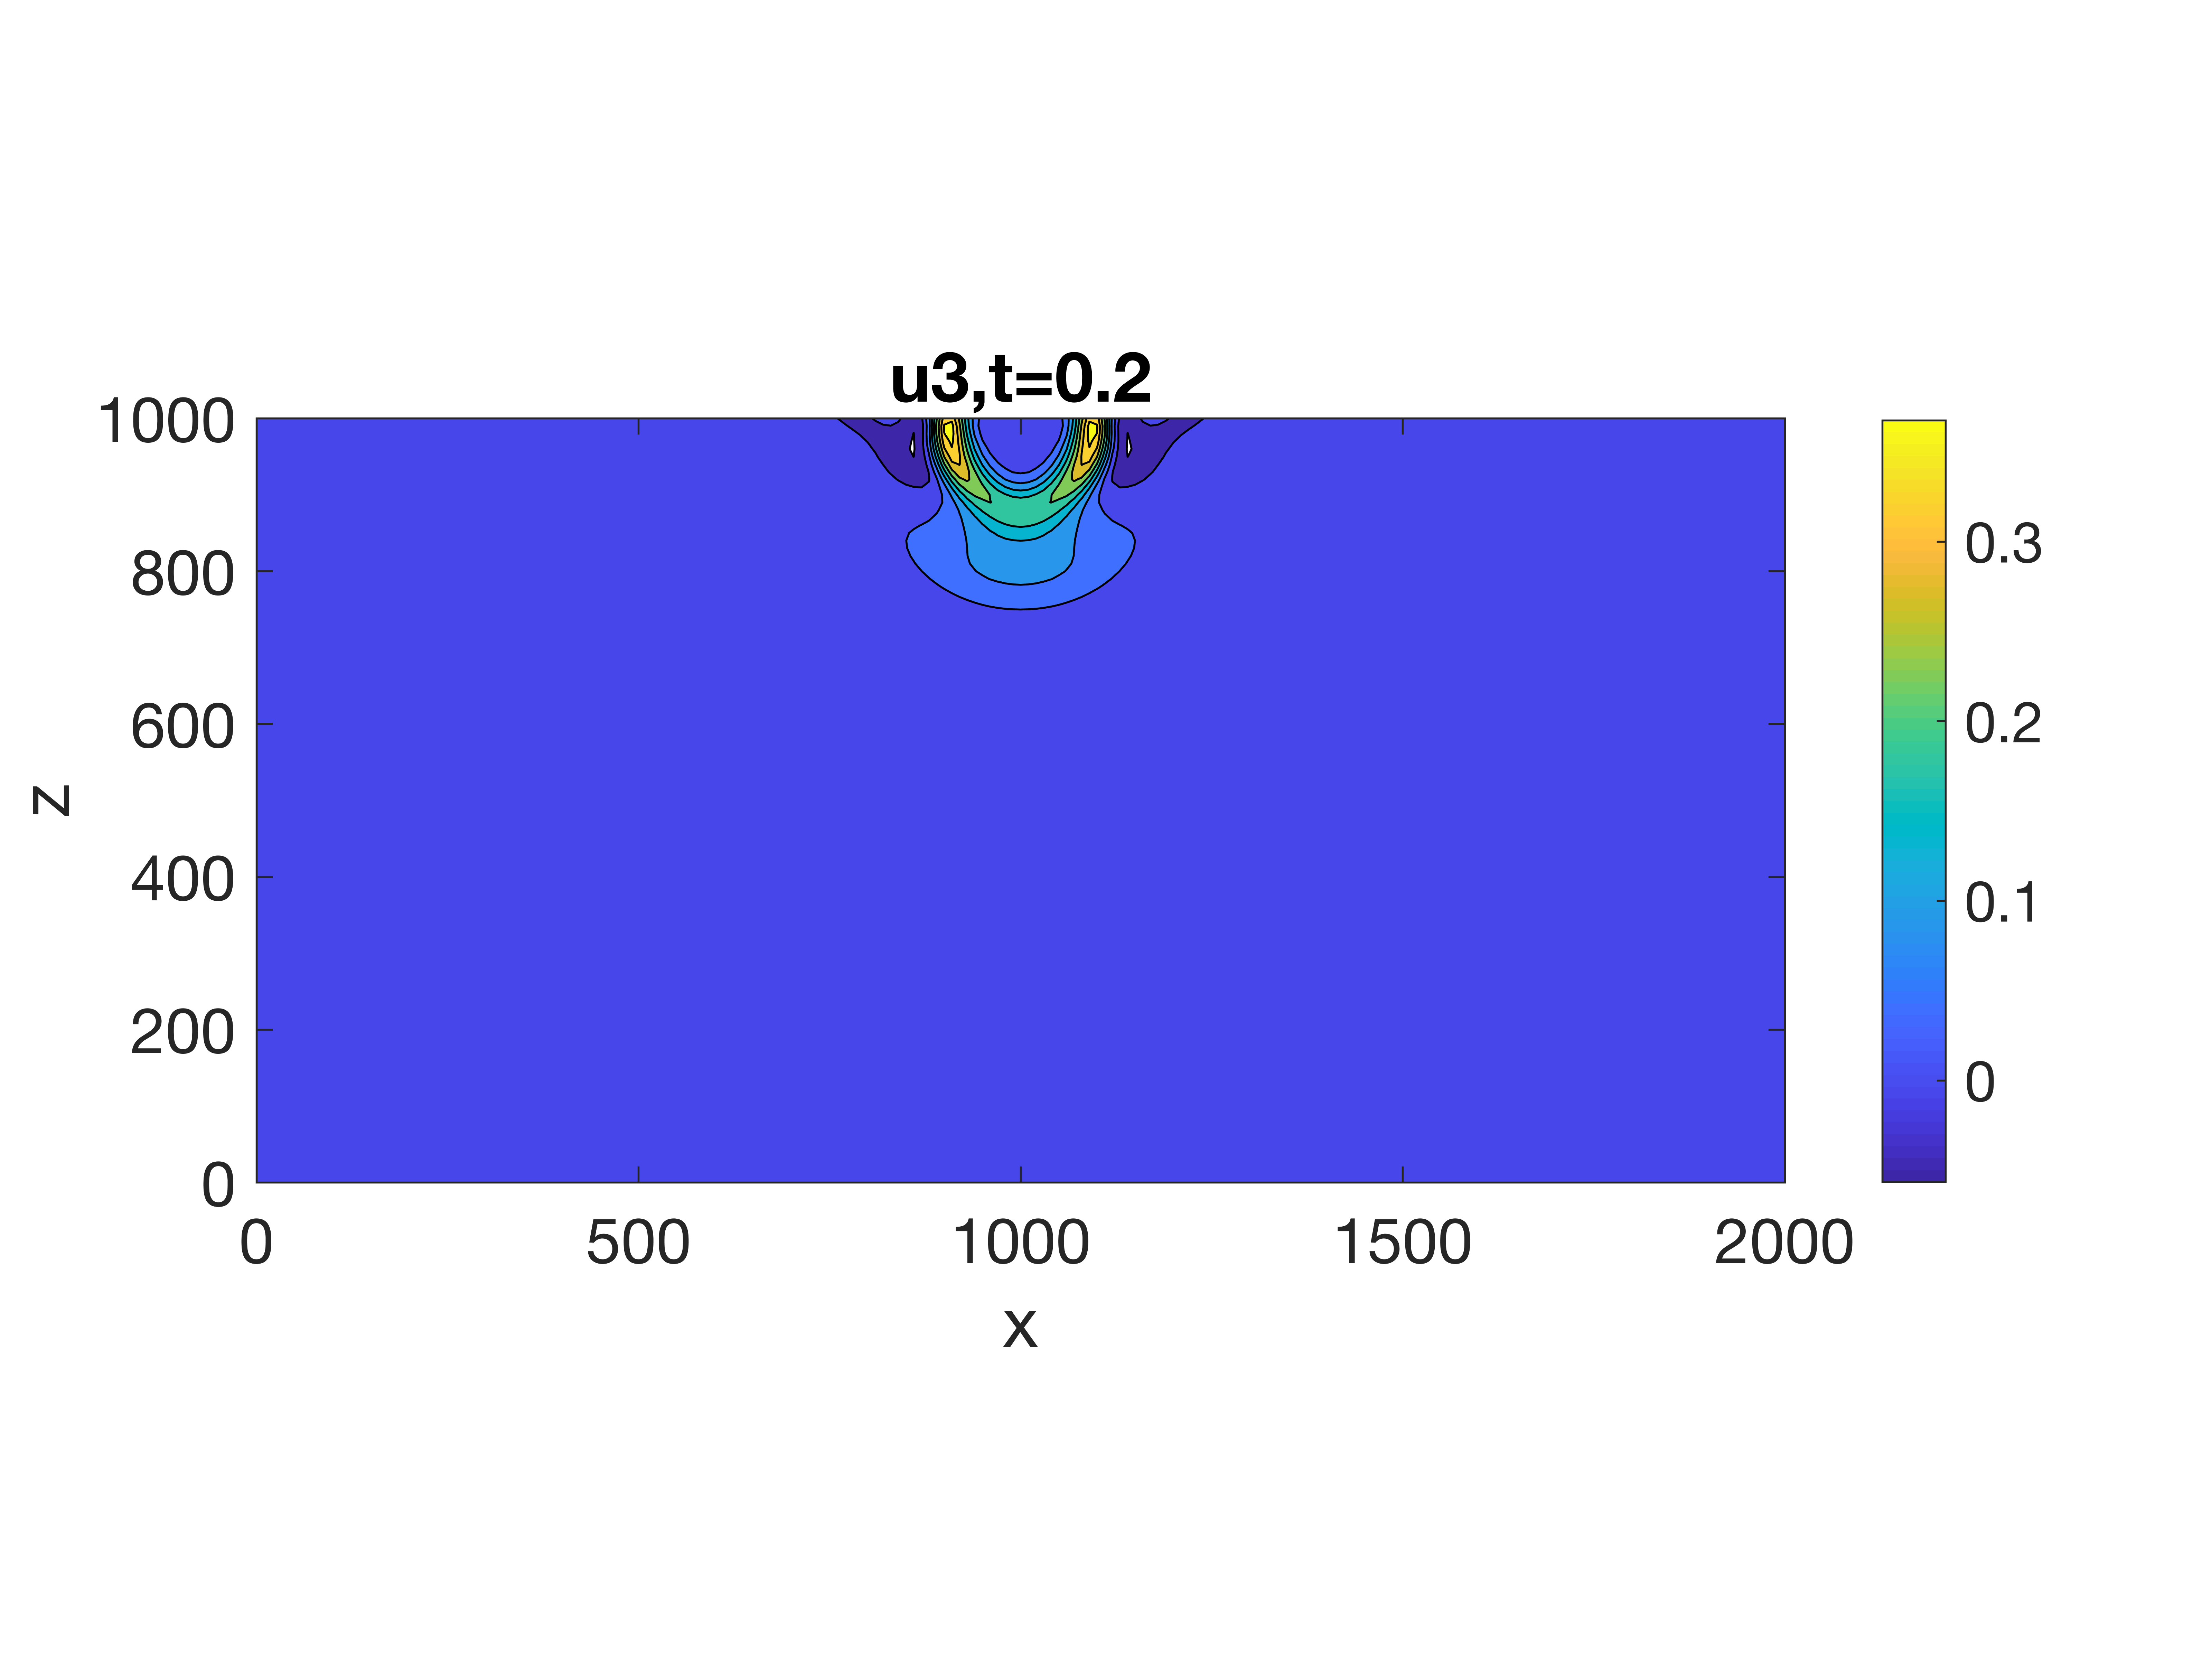
\includegraphics[width=0.4\textwidth,trim={0 2.8cm 0 2.8cm}, clip]{u3_t02_cartesian.png}
	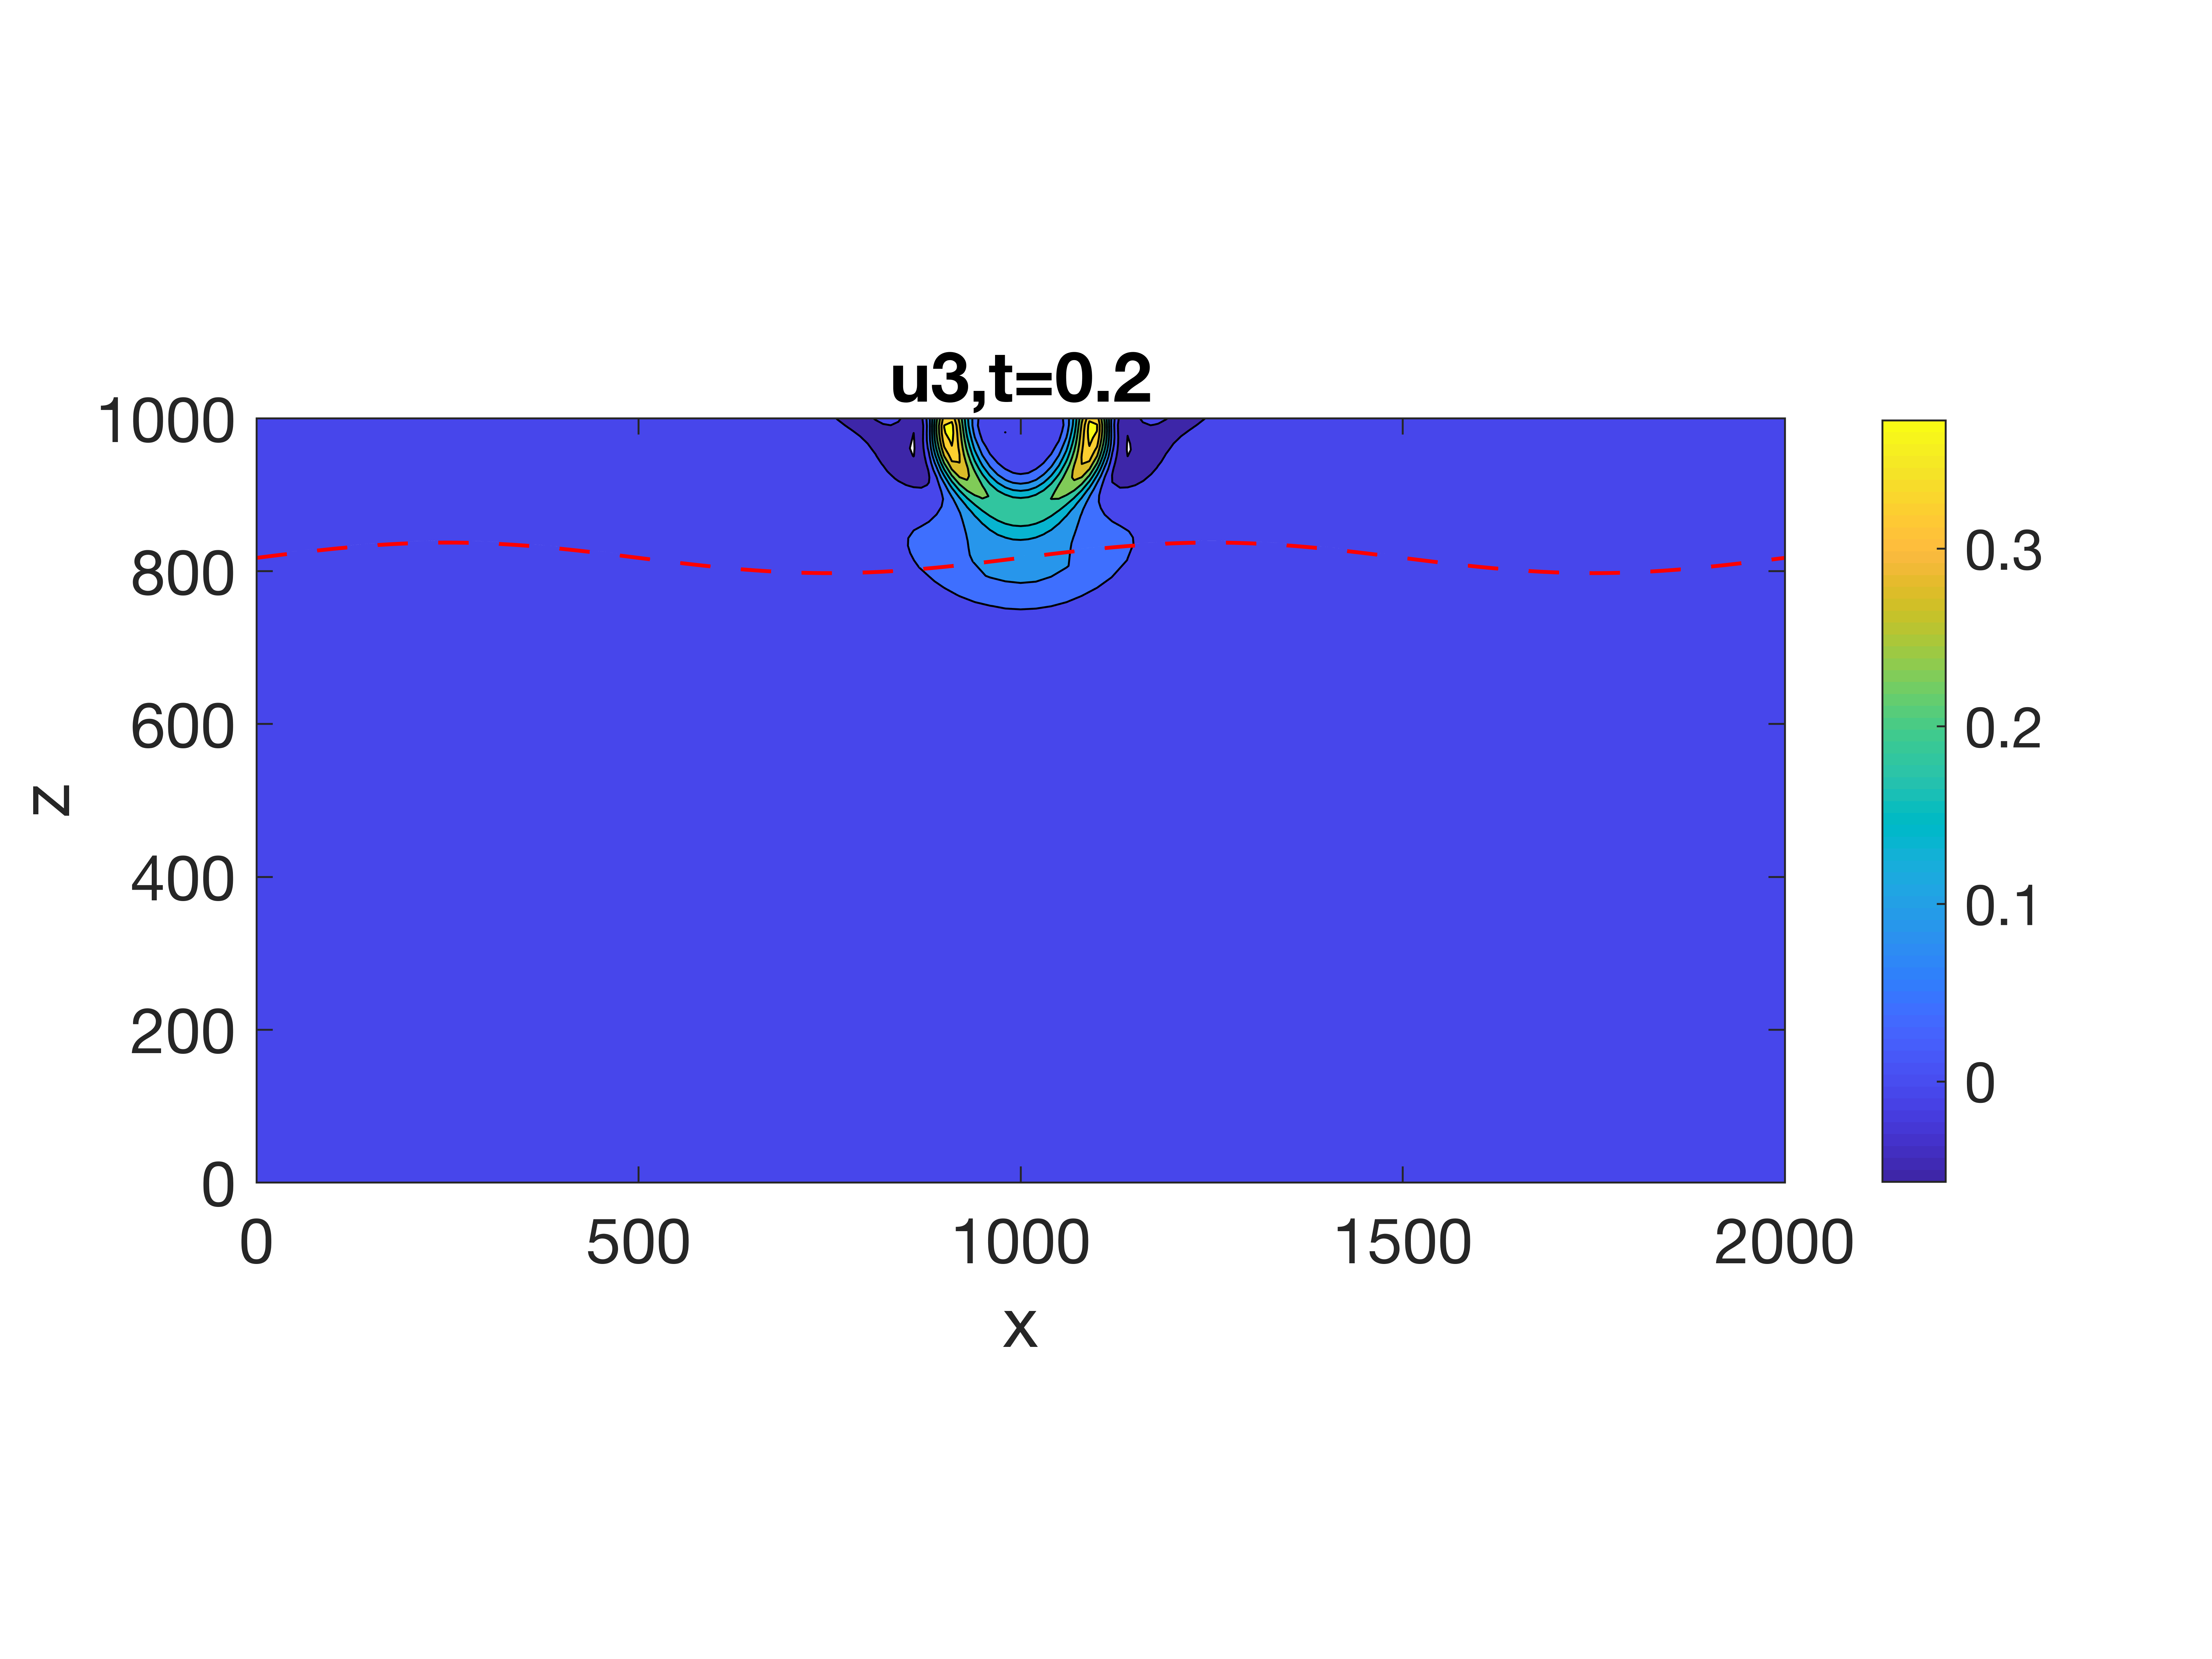
\includegraphics[width=0.4\textwidth,trim={0 2.8cm 0 2.8cm}, clip]{u3_t02_curvi_mr.png}\\
	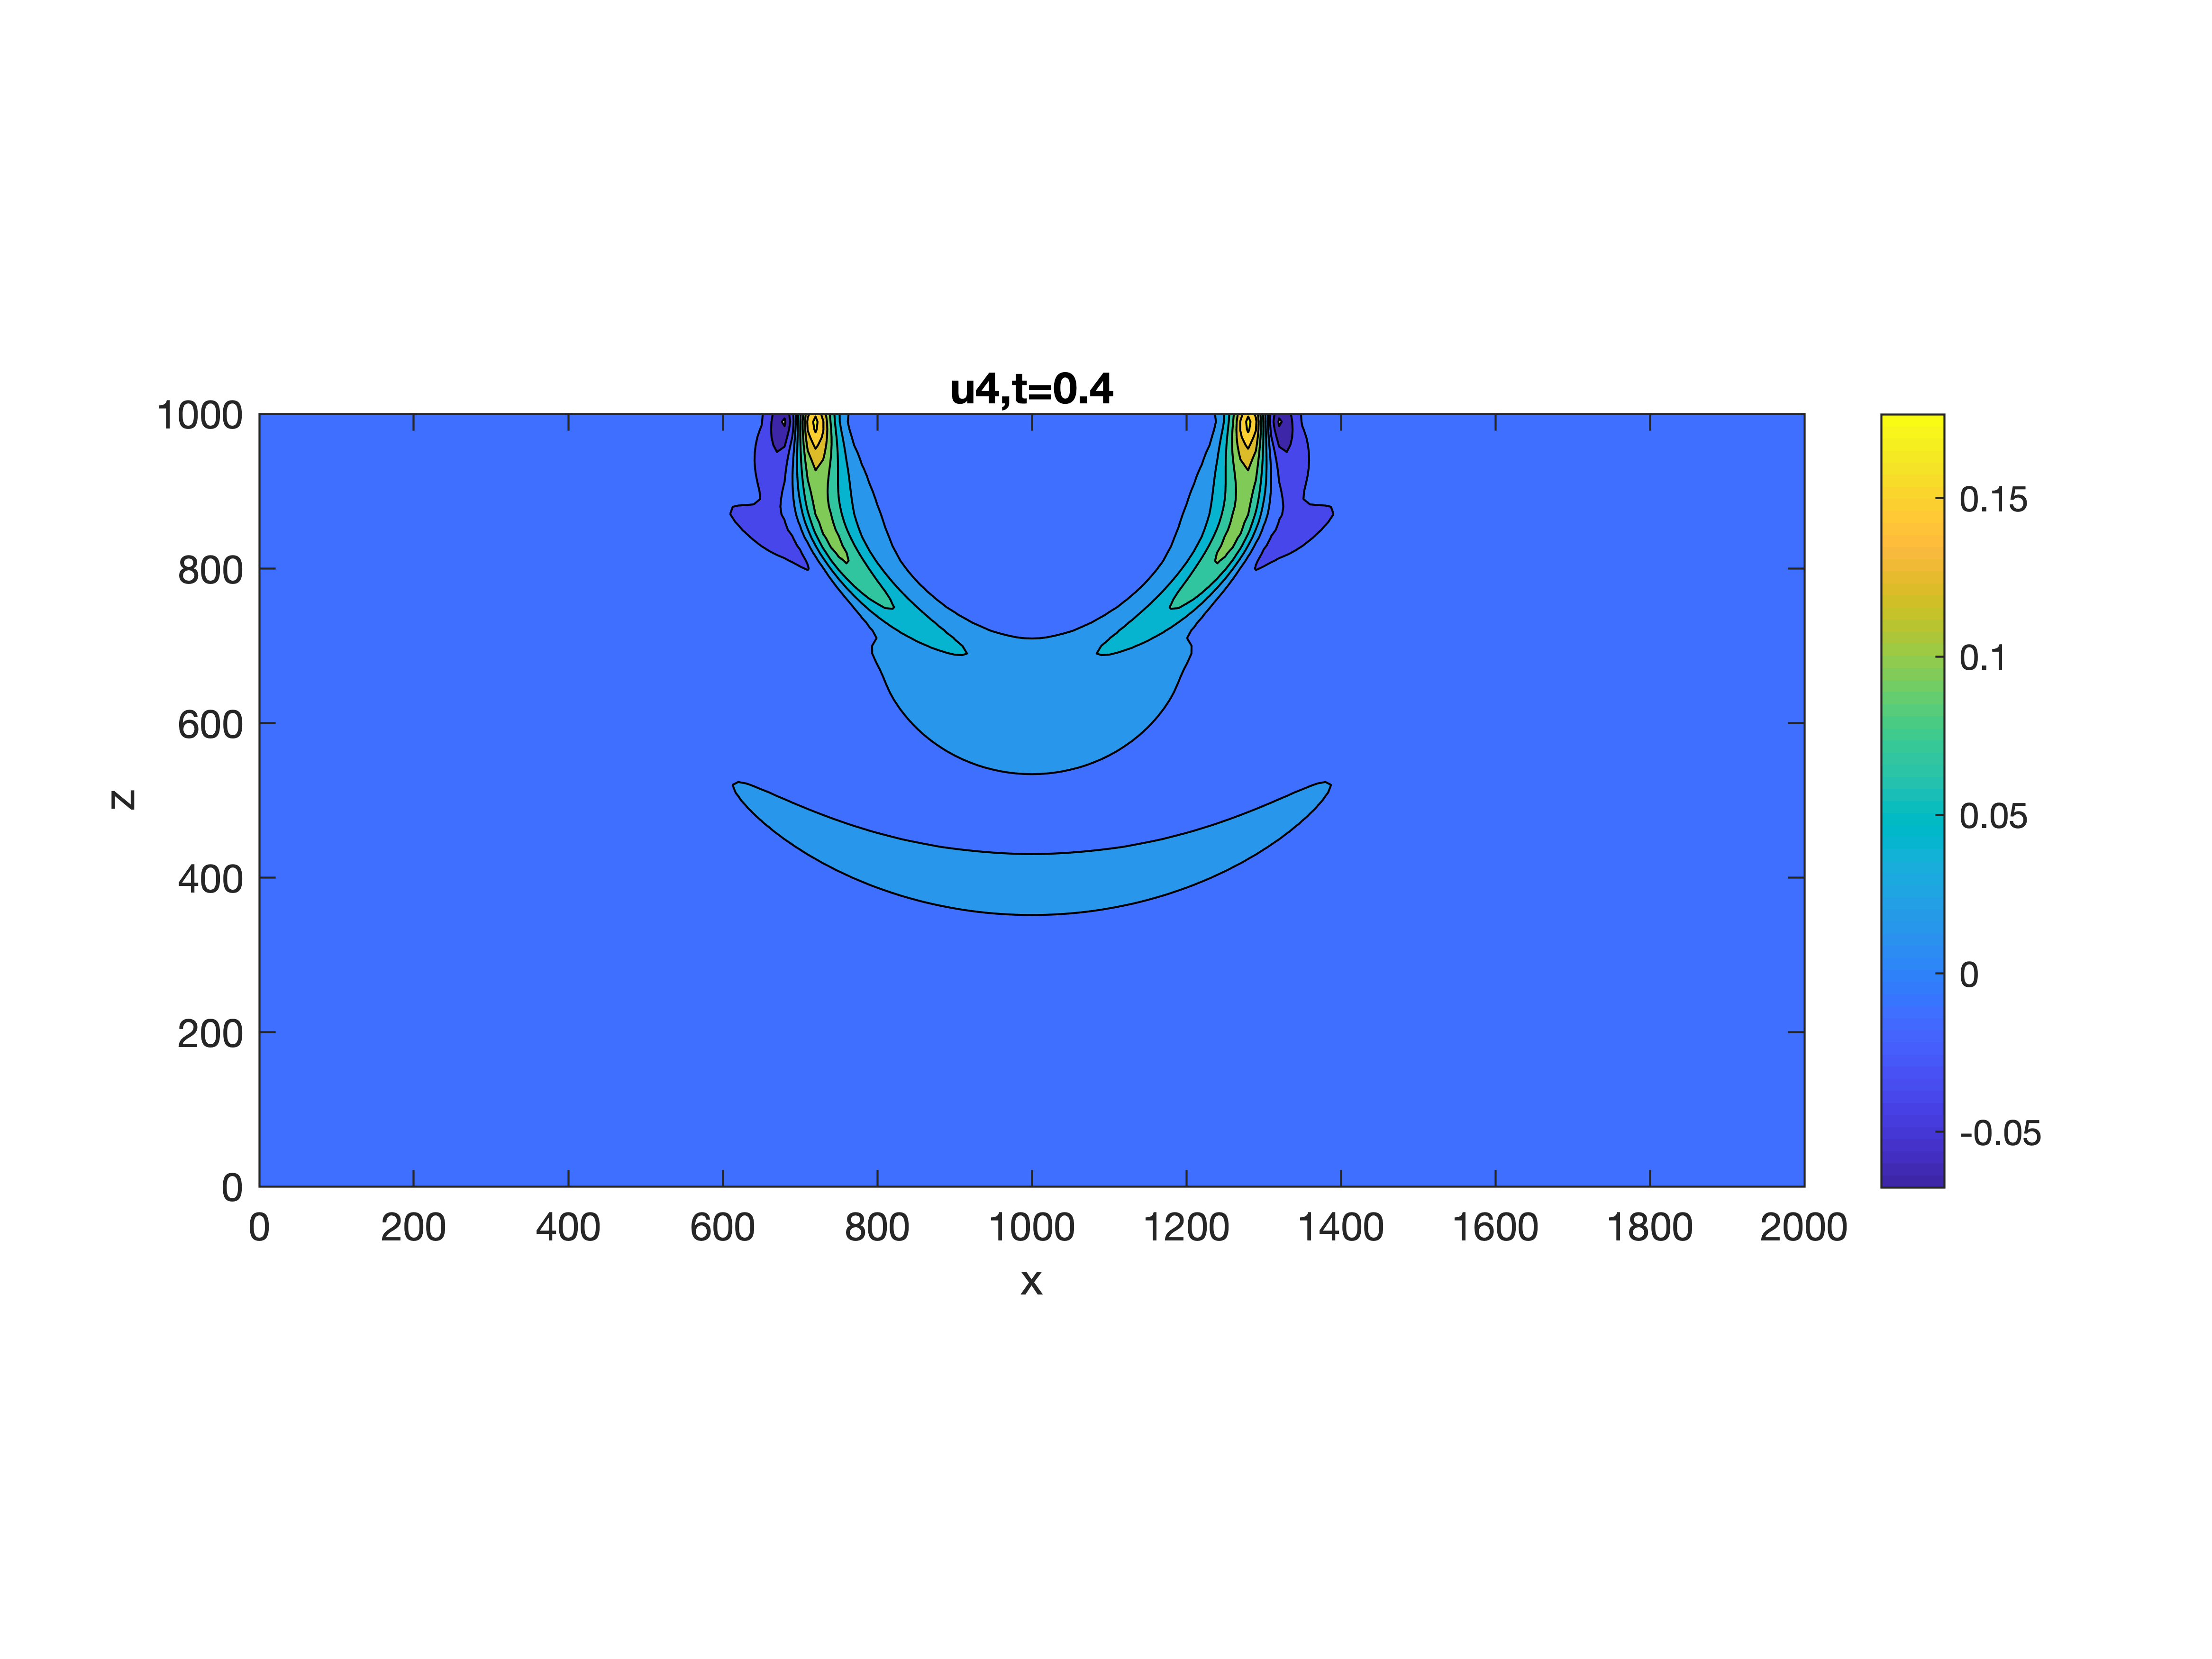
\includegraphics[width=0.4\textwidth,trim={0 2.8cm 0 2.8cm}, clip]{u3_t04_cartesian.png}
	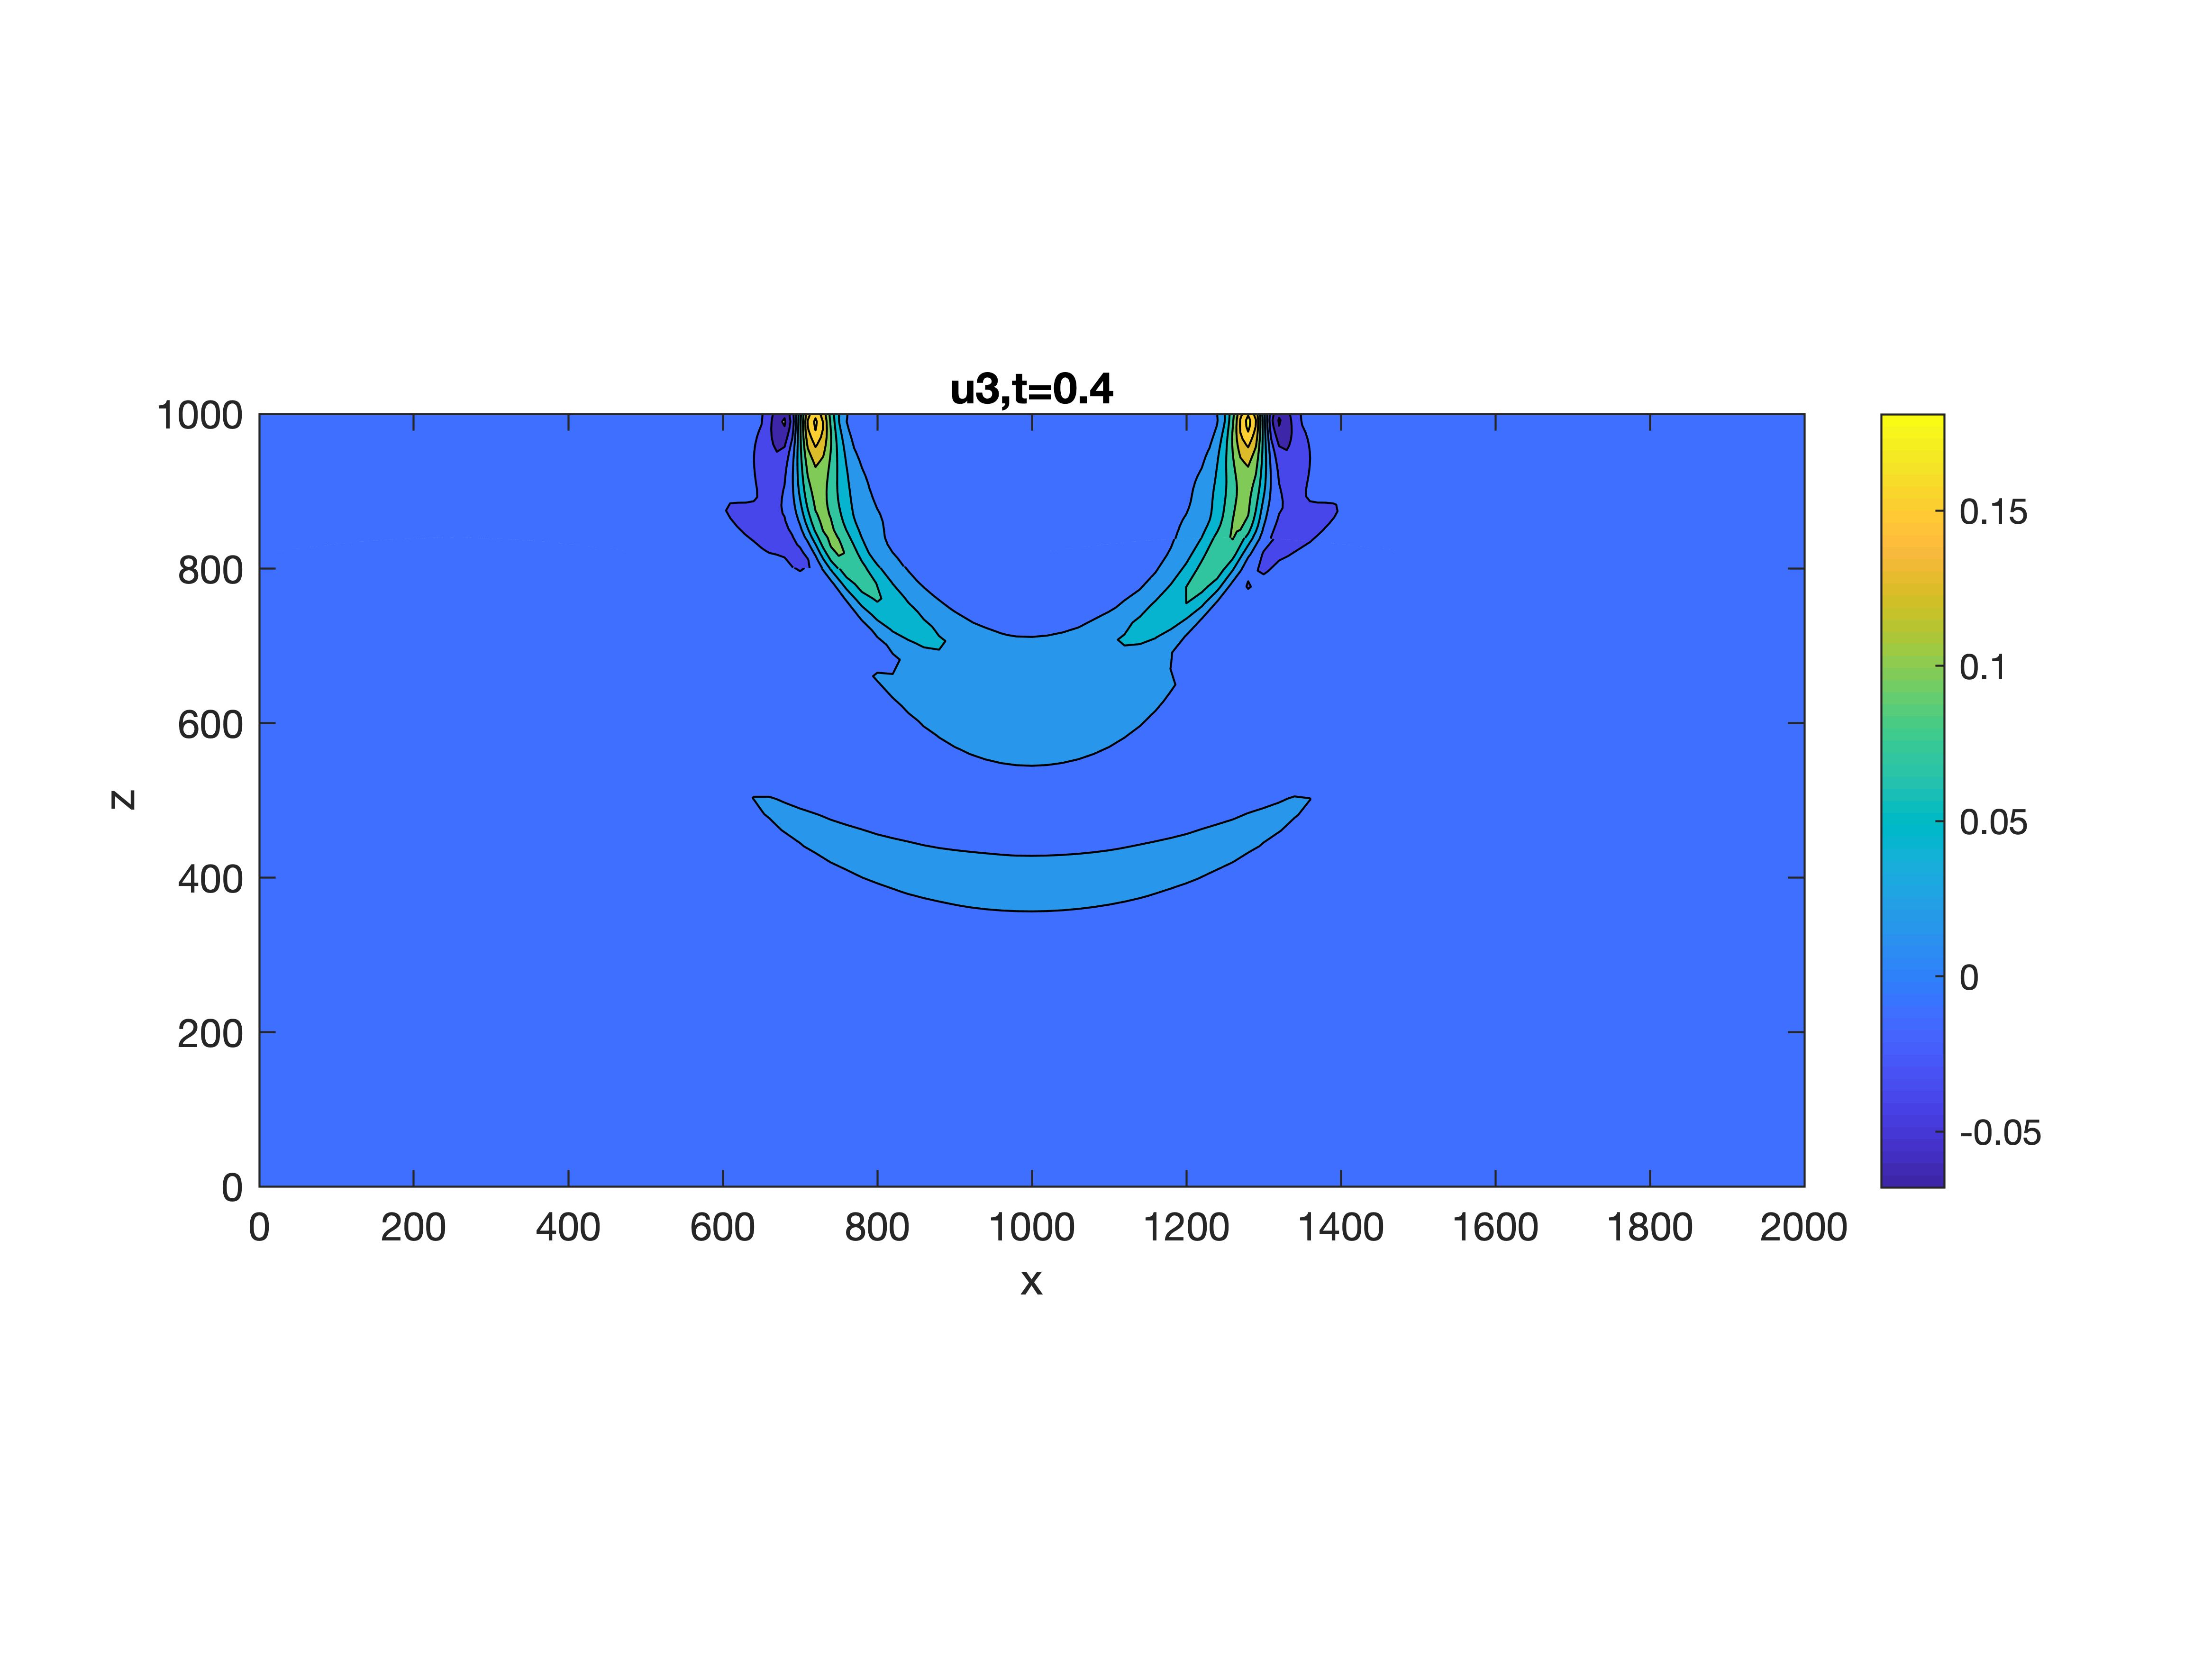
\includegraphics[width=0.4\textwidth,trim={0 2.8cm 0 2.8cm}, clip]{u3_t04_curvi_mr.png}
	\caption{The graphs for $u_3$. In the two figures on the left, we show reference solutions at $t=0.2$ and $t=0.4$, computed on a Cartesian mesh without mesh refinement interface. On the right, the two figures show the solutions computed on a curvilinear mesh with a curved mesh refinement interface at $t=0.2$ and $t=0.4$. The curved interfaces are marked with the red dash lines. Note that $x,z$ in the graph correspond to $x^{(1)}, x^{(3)}$ respectively.}
\label{u3}
\end{figure}
From Figure \ref{u1} and Figure \ref{u3}, we observe that there is no significant reflection at the mesh refinement interface for both component $u_1$ and $u_3$. As for component $u_2$, it is zero up to round-off error, and is not presented here.